\documentclass[12pt,a4paper]{report}

\usepackage{fontspec}
\setmainfont{Times New Roman}
\setsansfont{Arial}
\usepackage{polyglossia}
\setdefaultlanguage{vietnamese}

\usepackage[a4paper,left=3.0cm,right=2.2cm,top=2.5cm,bottom=2.5cm,headheight=15pt]{geometry}
\usepackage{graphicx}
\usepackage{booktabs}
\usepackage{longtable}
\usepackage{tabularx}
\usepackage{array}
\usepackage{multirow}
\usepackage{makecell}
\usepackage{enumitem}
\usepackage{float}
\usepackage{caption}
\usepackage[table]{xcolor}
\usepackage{fancyhdr}
\usepackage{titlesec}
\usepackage{tocloft}
\usepackage{hyperref}
\usepackage{bookmark}
\usepackage{microtype}
\usepackage{lastpage}

\definecolor{HUSTBlue}{HTML}{123A63}
\definecolor{HUSTLight}{HTML}{EAF1F8}
\definecolor{HUSTMid}{HTML}{D5E2EF}
\definecolor{TextGray}{HTML}{4B5563}
\definecolor{RuleGray}{HTML}{B8C5D1}

\hypersetup{
  colorlinks=true,
  linkcolor=HUSTBlue,
  urlcolor=HUSTBlue,
  citecolor=HUSTBlue,
  pdftitle={Báo cáo tổng hợp dự án Nhóm 1},
  pdfauthor={Nhóm 1}
}

\renewcommand{\chaptername}{Chương}
\titleformat{\chapter}[display]
  {\normalfont\sffamily\bfseries\color{HUSTBlue}}
  {\filleft\Large\chaptername\ \thechapter}
  {0.5ex}
  {\titlerule[1pt]\vspace{1ex}\Huge}
  [\vspace{1ex}\titlerule]
\titleformat{\section}
  {\normalfont\sffamily\bfseries\color{HUSTBlue}}
  {\thesection}{0.6em}{\Large}
\titleformat{\subsection}
  {\normalfont\sffamily\bfseries\color{HUSTBlue}}
  {\thesubsection}{0.6em}{\large}
\titleformat{\subsubsection}
  {\normalfont\sffamily\bfseries\color{HUSTBlue}}
  {\thesubsubsection}{0.6em}{\normalsize}

\setlength{\parindent}{1.0cm}
\setlength{\parskip}{0.35em}
\setlength{\emergencystretch}{3em}
\renewcommand{\arraystretch}{1.18}
\setlist[itemize]{leftmargin=1.0cm,itemsep=0.15em,topsep=0.2em}
\setlist[enumerate]{leftmargin=1.0cm,itemsep=0.15em,topsep=0.2em}
\setlist[description]{style=multiline,leftmargin=3.2cm,labelindent=0cm,itemsep=0.25em}

\newcolumntype{Y}{>{\raggedright\arraybackslash}X}
\newcolumntype{L}[1]{>{\raggedright\arraybackslash}p{#1}}
\newcolumntype{C}[1]{>{\centering\arraybackslash}p{#1}}
\newcommand{\tablehead}[1]{\cellcolor{HUSTBlue}\color{white}\textbf{#1}}
\newcommand{\sourceNote}[1]{\par\vspace{0.2em}\noindent{\footnotesize\itshape\color{TextGray}Nguồn trong hồ sơ Nhóm 1: #1.}}
\newcommand{\metric}[1]{\textbf{#1}}
\newcommand{\projectname}{Xây dựng hệ thống quản lý hàng hóa và kho bãi sản phẩm thời trang}
\newcommand{\projectcode}{CNTT20261\_N01}
\newcommand{\vnd}[1]{#1~VNĐ}

\pagestyle{fancy}
\fancyhf{}
\fancyhead[L]{\small\sffamily\color{TextGray}Báo cáo tổng hợp dự án}
\fancyhead[R]{\small\sffamily\color{TextGray}Nhóm 1}
\fancyfoot[C]{\small\thepage/\pageref{LastPage}}
\renewcommand{\headrulewidth}{0.4pt}
\renewcommand{\headrule}{\hbox to\headwidth{\color{RuleGray}\leaders\hrule height \headrulewidth\hfill}}

\captionsetup{
  font=small,
  labelfont={bf,color=HUSTBlue},
  labelsep=period,
  justification=raggedright,
  singlelinecheck=false
}

\begin{document}

\begin{titlepage}
\thispagestyle{empty}
\centering

\includegraphics[height=3.4cm]{assets/logo.png}\par
\vspace{0.7cm}
{\Large\bfseries ĐẠI HỌC BÁCH KHOA HÀ NỘI\par}
\vspace{0.15cm}
{\large\bfseries TRƯỜNG CÔNG NGHỆ THÔNG TIN VÀ TRUYỀN THÔNG\par}
\vspace{1.4cm}
\rule{\textwidth}{1pt}\par
\vspace{0.35cm}
{\Huge\bfseries\color{HUSTBlue} BÁO CÁO TỔNG HỢP DỰ ÁN\par}
\vspace{0.35cm}
\rule{\textwidth}{1pt}\par
\vspace{1.0cm}
{\Large\bfseries \projectname\par}
\vspace{1.0cm}
\begin{tabular}{rl}
\textbf{Mã dự án:} & \projectcode\\[0.25cm]
\textbf{Thời gian:} & 01/09/2026 - 31/03/2027\\[0.25cm]
\textbf{Giám đốc dự án:} & Bùi Tuấn Anh\\[0.25cm]
\textbf{Giảng viên hướng dẫn:} & ThS. Lê Thị Hoa
\end{tabular}
\vfill
\begin{tabular}{ll}
\textbf{Nhóm 1} & \textbf{Mã sinh viên}\\
Bùi Tuấn Anh & 202490032\\
Bùi Quốc Luýt & 202490069\\
Vũ Quang Minh & 202490071\\
Bạch Minh Quang & 202490077\\
Phạm Đoàn Bảo Thiên & 202490090
\end{tabular}
\vfill
{\large Hà Nội, tháng 9 năm 2026\par}
\end{titlepage}

\pagenumbering{roman}
\chapter*{Tóm tắt}
\addcontentsline{toc}{chapter}{Tóm tắt}

Báo cáo này tổng hợp bộ hồ sơ dự án của Nhóm 1 về hệ thống quản lý hàng hóa và kho bãi sản phẩm thời trang. Nội dung được hợp nhất từ báo cáo khảo sát, báo cáo phân tích và thiết kế hệ thống, tôn chỉ và bảng phân rã công việc, bảng dự toán kinh phí và kế hoạch quản lý chất lượng. Báo cáo không sử dụng slide, tệp Microsoft Project hoặc tệp được đánh dấu old - delete.

Hồ sơ mô tả một doanh nghiệp kinh doanh thời trang có kho tổng, kho tại cửa hàng, nhiều nhà cung cấp và nhiều kênh bán hàng. Vấn đề trung tâm là tồn kho phải được quản lý theo từng biến thể sản phẩm, tức tổ hợp sản phẩm, màu sắc và kích thước. Từ hiện trạng quản lý bằng sổ sách và nhiều tệp Excel rời rạc, nhóm xác định phạm vi hệ thống, 19 yêu cầu chức năng, 11 yêu cầu phi chức năng, 19 use case, kiến trúc web ba tầng, 15 bảng dữ liệu và 10 màn hình nghiệp vụ.

Về quản lý dự án, kế hoạch kéo dài từ ngày 01/09/2026 đến ngày 31/03/2027, gồm sáu giai đoạn và 52 task. Tổng khối lượng chốt trong WBS là khoảng 221,83 manday. Dự toán kinh phí là 408.196.650 VNĐ, gồm công lao động, vật tư thiết bị và các khoản chi khác. Kế hoạch chất lượng quy định các mốc kiểm soát, trách nhiệm, cách kiểm thử, quản lý lỗi và điều kiện nghiệm thu.

\chapter*{Phạm vi tổng hợp}
\addcontentsline{toc}{chapter}{Phạm vi tổng hợp}

\begin{tabularx}{\textwidth}{L{0.8cm}Y}
\toprule
\tablehead{STT} & \tablehead{Tài liệu được sử dụng}\\
\midrule
1 & \texttt{Nhóm 1 - Báo cáo khảo sát.docx}\\
2 & \texttt{bao-cao-phan-tich-thiet-ke.docx}\\
3 & \texttt{quan-ly-chat-luong.docx}\\
4 & \texttt{ton-chi-DA-va-phan-ra-cong-viec.xlsx}\\
5 & \texttt{kinh-phi-du-an.xlsx}\\
\bottomrule
\end{tabularx}

\vspace{0.4em}
Các con số, tên người, mốc thời gian, yêu cầu và mô tả kỹ thuật trong báo cáo đều lấy từ năm tài liệu trên hoặc là phép tổng hợp trực tiếp của các số liệu đó. Khi nguồn mô tả mục tiêu ở mức khác với tiêu chí kiểm thử chi tiết, báo cáo giữ cả hai mức và ghi rõ ngữ cảnh.

\tableofcontents
\listoftables
\listoffigures

\clearpage
\pagenumbering{arabic}

\chapter{Tổng quan dự án và tôn chỉ}

\section{Thông tin chung}

\begin{table}[H]
\centering
\caption{Thông tin chính của dự án}
\begin{tabularx}{\textwidth}{L{4.2cm}Y}
\toprule
\tablehead{Nội dung} & \tablehead{Thông tin}\\
\midrule
Tên dự án & \projectname\\
Mã số & \projectcode\\
Chủ đầu tư & Doanh nghiệp kinh doanh sản phẩm thời trang, là đơn vị được khảo sát\\
Thời gian & 01/09/2026 - 31/03/2027, tương ứng 07 tháng\\
Giám đốc dự án & Bùi Tuấn Anh\\
Trưởng nhóm kỹ thuật & Bùi Quốc Luýt\\
Quy mô & Dự án phần mềm quy mô vừa, gồm 5 thành viên\\
Kinh phí phê duyệt & \vnd{408.196.650}\\
\bottomrule
\end{tabularx}
\end{table}

\section{Thành viên và trách nhiệm}

\begin{table}[H]
\centering
\caption{Thành viên dự án}
\small
\begin{tabularx}{\textwidth}{L{3.8cm}L{2.2cm}Y}
\toprule
\tablehead{Thành viên} & \tablehead{Mã sinh viên} & \tablehead{Vai trò và trách nhiệm chính}\\
\midrule
Bùi Tuấn Anh & 202490032 & Giám đốc dự án, phân tích nghiệp vụ; chủ trì rà soát yêu cầu, UAT, nghiệm thu và báo cáo.\\
Bùi Quốc Luýt & 202490069 & Trưởng nhóm kỹ thuật, back-end; rà soát kiến trúc, thiết kế lớp, pull request và điều phối sửa lỗi.\\
Vũ Quang Minh & 202490071 & Lập trình back-end; viết unit test cho nghiệp vụ kho, kiểm kê, đổi trả và hủy hàng.\\
Bạch Minh Quang & 202490077 & Thiết kế UI/UX, front-end; bảo đảm giao diện trên máy tính bảng và máy quét mã vạch, kiểm thử phân quyền trên giao diện.\\
Phạm Đoàn Bảo Thiên & 202490090 & Thiết kế cơ sở dữ liệu, kiểm thử; phụ trách bộ test case, kiểm thử kho, đồng thời và hiệu năng.\\
\bottomrule
\end{tabularx}
\end{table}

\section{Mục tiêu dự án}

Mục tiêu tổng quát là xây dựng hệ thống phần mềm quản lý tập trung hàng hóa và kho bãi cho doanh nghiệp kinh doanh thời trang, thay thế việc quản lý bằng sổ sách và nhiều tệp Excel rời rạc. Hệ thống lấy kho làm trung tâm và quản lý tồn đến từng biến thể, tức sản phẩm kết hợp với màu và size.

\begin{enumerate}
\item Tồn kho của mọi biến thể tại mọi kho được cập nhật khi phiếu kho hoàn tất; sai lệch giữa tồn hệ thống và tồn thực tế sau kiểm kê định kỳ dưới 1\%.
\item Không thể xuất kho vượt quá số lượng tồn, kể cả khi nhiều yêu cầu xuất được xử lý đồng thời.
\item Truy xuất được lịch sử biến động của một biến thể theo người thực hiện, thời gian, chứng từ và số lượng thay đổi trong vài giây.
\item Rút thời gian lập báo cáo nhập - xuất - tồn tháng từ khoảng một ngày làm việc xuống dưới 1 phút.
\item Cảnh báo tự động các biến thể hết hàng hoặc sắp hết để hỗ trợ quản lý nhập bổ sung.
\end{enumerate}

\noindent\textbf{Đối chiếu chỉ tiêu:} mục tiêu cấp dự án nêu thời gian lập báo cáo dưới 1 phút. NFR-02 và tiêu chí kiểm thử chi tiết trong hồ sơ thiết kế nêu thời gian báo cáo một tháng dưới 10 giây. Hai mức này được giữ nguyên trong báo cáo vì thuộc hai lớp mục tiêu khác nhau.

\section{Phạm vi}

\begin{table}[H]
\centering
\caption{Phạm vi trong và ngoài dự án}
\small
\begin{tabularx}{\textwidth}{Y Y}
\toprule
\tablehead{Trong phạm vi} & \tablehead{Ngoài phạm vi}\\
\midrule
Quản lý tài khoản, vai trò và kho phụ trách. & Bán hàng tại quầy, thanh toán và hóa đơn điện tử.\\
Quản lý sản phẩm, biến thể, loại, màu, size, nhà cung cấp, kho và vị trí. & Đặt hàng với nhà cung cấp, công nợ và kế toán giá vốn.\\
Nhập, xuất, chuyển kho, đổi trả, hủy hàng. & Kết nối sàn thương mại điện tử và đơn vị vận chuyển.\\
Kiểm kê và điều chỉnh tồn có phê duyệt. & Chăm sóc khách hàng và chương trình khuyến mãi.\\
Tra cứu tồn, cảnh báo, báo cáo, thẻ kho, chuyển đổi tồn đầu kỳ, triển khai, đào tạo và bàn giao. & Ứng dụng di động riêng và mua sắm thiết bị phần cứng.\\
\bottomrule
\end{tabularx}
\end{table}

\section{Quy tắc nghiệp vụ cốt lõi}

\begin{enumerate}[label=\textbf{QT-\arabic*:},leftmargin=1.35cm]
\item Tồn kho được quản lý theo cặp (kho, biến thể); số lượng tồn không âm.
\item Tồn kho chỉ thay đổi khi phiếu kho chuyển sang trạng thái Hoàn thành; phiếu đang lập hoặc chờ duyệt không ảnh hưởng tồn.
\item Chênh lệch kiểm kê bằng số lượng thực tế trừ tồn hệ thống tại thời điểm kiểm kê; mọi điều chỉnh tồn phải được Quản lý duyệt.
\item Hàng trả tình trạng Còn tốt được nhập lại kho bán; hàng lỗi, hỏng vào kho hàng lỗi và không làm tăng tồn có thể bán.
\item Biến thể Hết hàng khi tồn bằng 0, Sắp hết khi tồn lớn hơn 0 và không vượt tồn tối thiểu, Bình thường khi tồn lớn hơn tồn tối thiểu.
\item Tồn cuối kỳ bằng tồn đầu kỳ cộng nhập trừ xuất cộng hoặc trừ điều chỉnh. Nhập gồm nhập mua, nhận chuyển kho và hàng trả nhập lại; xuất gồm bán, chuyển đi, hủy và hàng đổi sang.
\end{enumerate}

\chapter{Khảo sát hiện trạng}

\section{Đặc thù bài toán}

Doanh nghiệp được khảo sát kinh doanh áo, quần, váy và áo khoác, với một kho tổng và các kho tại cửa hàng. Hàng hóa nhập từ nhiều nhà cung cấp và được bán tại cửa hàng hoặc qua kênh trực tuyến. Đặc thù quan trọng nhất là một mẫu có nhiều tổ hợp màu sắc và kích thước, vì vậy đơn vị quản lý tồn không chỉ là mẫu sản phẩm mà là biến thể.

Ví dụ, mẫu Áo thun AT01 có các biến thể Đen/S 1.000 sản phẩm, Đen/M 1.500 sản phẩm, Đen/L 800 sản phẩm, Trắng/S 1.200 sản phẩm và Trắng/M 2.000 sản phẩm. Tổng tồn của mẫu là 6.500 sản phẩm, nhưng tổng này không cho biết riêng biến thể Đen/M còn đủ cho một đơn hàng hay không.

\section{Quy trình hiện tại}

\subsection{Nhập hàng}
Nhân viên nhận hàng từ nhà cung cấp, kiểm tra số lượng, mẫu mã, màu và size, đối chiếu với đơn đặt hàng hoặc hóa đơn, ghi nhận hàng nhập, sắp xếp vào vị trí và cập nhật tồn.

\subsection{Xuất hàng}
Kho nhận yêu cầu xuất từ bộ phận bán hàng hoặc đơn hàng, kiểm tra tồn, lấy hàng, kiểm tra sản phẩm, ghi nhận thông tin xuất và cập nhật lại số lượng.

\subsection{Kiểm kê}
Nhân viên đếm số lượng thực tế, đối chiếu với sổ sách hoặc tệp quản lý, xác định chênh lệch, điều chỉnh nếu cần và lập báo cáo kiểm kê.

\subsection{Đổi trả và nghiệp vụ phụ}
Khi đổi trả, nhân viên tiếp nhận hàng, kiểm tra tình trạng, xác định có thể nhập lại kho hay không, cập nhật tồn và ghi nhận nguyên nhân. Ngoài bốn quy trình cốt lõi, hồ sơ còn ghi nhận chuyển hàng giữa các kho và hủy hàng lỗi, hỏng hoặc không còn khả năng bán.

\section{Thông tin và biểu mẫu}

Thông tin hiện trạng gồm mã và tên sản phẩm, loại, màu, size, giá nhập, giá bán, nhà cung cấp, số lượng tồn, vị trí và trạng thái. Báo cáo phân tích xác định màu, size, giá và tồn phải được quản lý ở cấp biến thể; tồn phải gắn với từng biến thể tại từng kho.

\begin{longtable}{L{0.7cm}L{4.0cm}L{3.0cm}L{7.0cm}}
\caption{13 biểu mẫu nghiệp vụ được thu thập}\label{tab:forms}\\
\toprule
\tablehead{STT} & \tablehead{Biểu mẫu} & \tablehead{Nghiệp vụ} & \tablehead{Thông tin chính}\\
\midrule
\endfirsthead
\toprule
\tablehead{STT} & \tablehead{Biểu mẫu} & \tablehead{Nghiệp vụ} & \tablehead{Thông tin chính}\\
\midrule
\endhead
1 & Phiếu nhập kho & Nhập hàng & Mã phiếu, ngày, nhà cung cấp, kho nhập, dòng hàng.\\
2 & Phiếu xuất kho & Xuất hàng & Mã phiếu, kho xuất, người nhận, lý do và dòng hàng.\\
3 & Phiếu kiểm kê kho & Kiểm kê & Kho, phạm vi, tồn hệ thống, thực tế và chênh lệch.\\
4 & Phiếu điều chỉnh tồn kho & Điều chỉnh & Tồn trước, số điều chỉnh, tồn sau, lý do và người duyệt.\\
5 & Phiếu đổi/trả hàng & Đổi trả & Đơn hàng, khách hàng, lý do, tình trạng, hàng đổi và tiền chênh lệch.\\
6 & Phiếu chuyển kho & Chuyển kho & Kho xuất, kho nhận, người chuyển và người nhận.\\
7 & Phiếu hủy hàng & Hủy hàng & Kho, lý do hủy từng dòng và người duyệt.\\
8 & Báo cáo tồn kho & Tồn kho & Tồn theo sản phẩm, màu, size, kho và trạng thái.\\
9 & Báo cáo nhập kho & Nhập kho & Theo thời gian, nhà cung cấp, sản phẩm; tổng phiếu, số lượng và giá trị.\\
10 & Báo cáo xuất kho & Xuất kho & Theo thời gian, lý do xuất, sản phẩm và kho.\\
11 & Báo cáo nhập - xuất - tồn & Tổng hợp & Tồn cuối = tồn đầu + nhập - xuất cộng hoặc trừ điều chỉnh.\\
12 & Báo cáo kiểm kê & Kiểm kê & Chênh lệch, nguyên nhân, tổng thiếu/thừa và giá trị chênh lệch.\\
13 & Báo cáo biến động hàng hóa & Truy xuất & Lịch sử từng lần thay đổi số lượng của một biến thể.\\
\bottomrule
\end{longtable}

\section{Các vấn đề và nhu cầu hệ thống}

\begin{table}[H]
\centering
\caption{Vấn đề hiện tại và nhu cầu được xác định}
\small
\begin{tabularx}{\textwidth}{Y Y}
\toprule
\tablehead{Vấn đề hiện tại} & \tablehead{Nhu cầu hệ thống}\\
\midrule
Dữ liệu phân tán ở nhiều tệp, không đồng nhất. & Tập trung dữ liệu trên một hệ thống duy nhất.\\
Khó quản lý nhiều biến thể màu và size. & Quản lý từng biến thể và sinh mã SKU.\\
Tồn kho sai lệch, không theo thời gian thực. & Tự động cập nhật tồn khi phiếu hoàn tất.\\
Khó kiểm tra lịch sử biến động. & Lưu thẻ kho cho mọi thay đổi số lượng.\\
Tìm kiếm thông tin mất thời gian. & Tìm kiếm, lọc theo sản phẩm, màu, size và kho.\\
Kiểm kê và đối chiếu thủ công. & Tự tính chênh lệch và điều chỉnh có phê duyệt.\\
Báo cáo phải lập thủ công. & Tự động tổng hợp các báo cáo kho.\\
Khó kiểm soát thao tác nhân viên. & Phân quyền theo vai trò và ghi nhận người thực hiện.\\
Khó phát hiện hàng sắp hết. & Cảnh báo tồn kho thấp.\\
Không phát hiện hàng tồn lâu. & Theo dõi số ngày tồn và hỗ trợ quyết định xử lý.\\
\bottomrule
\end{tabularx}
\end{table}

\begin{figure}[H]
\centering
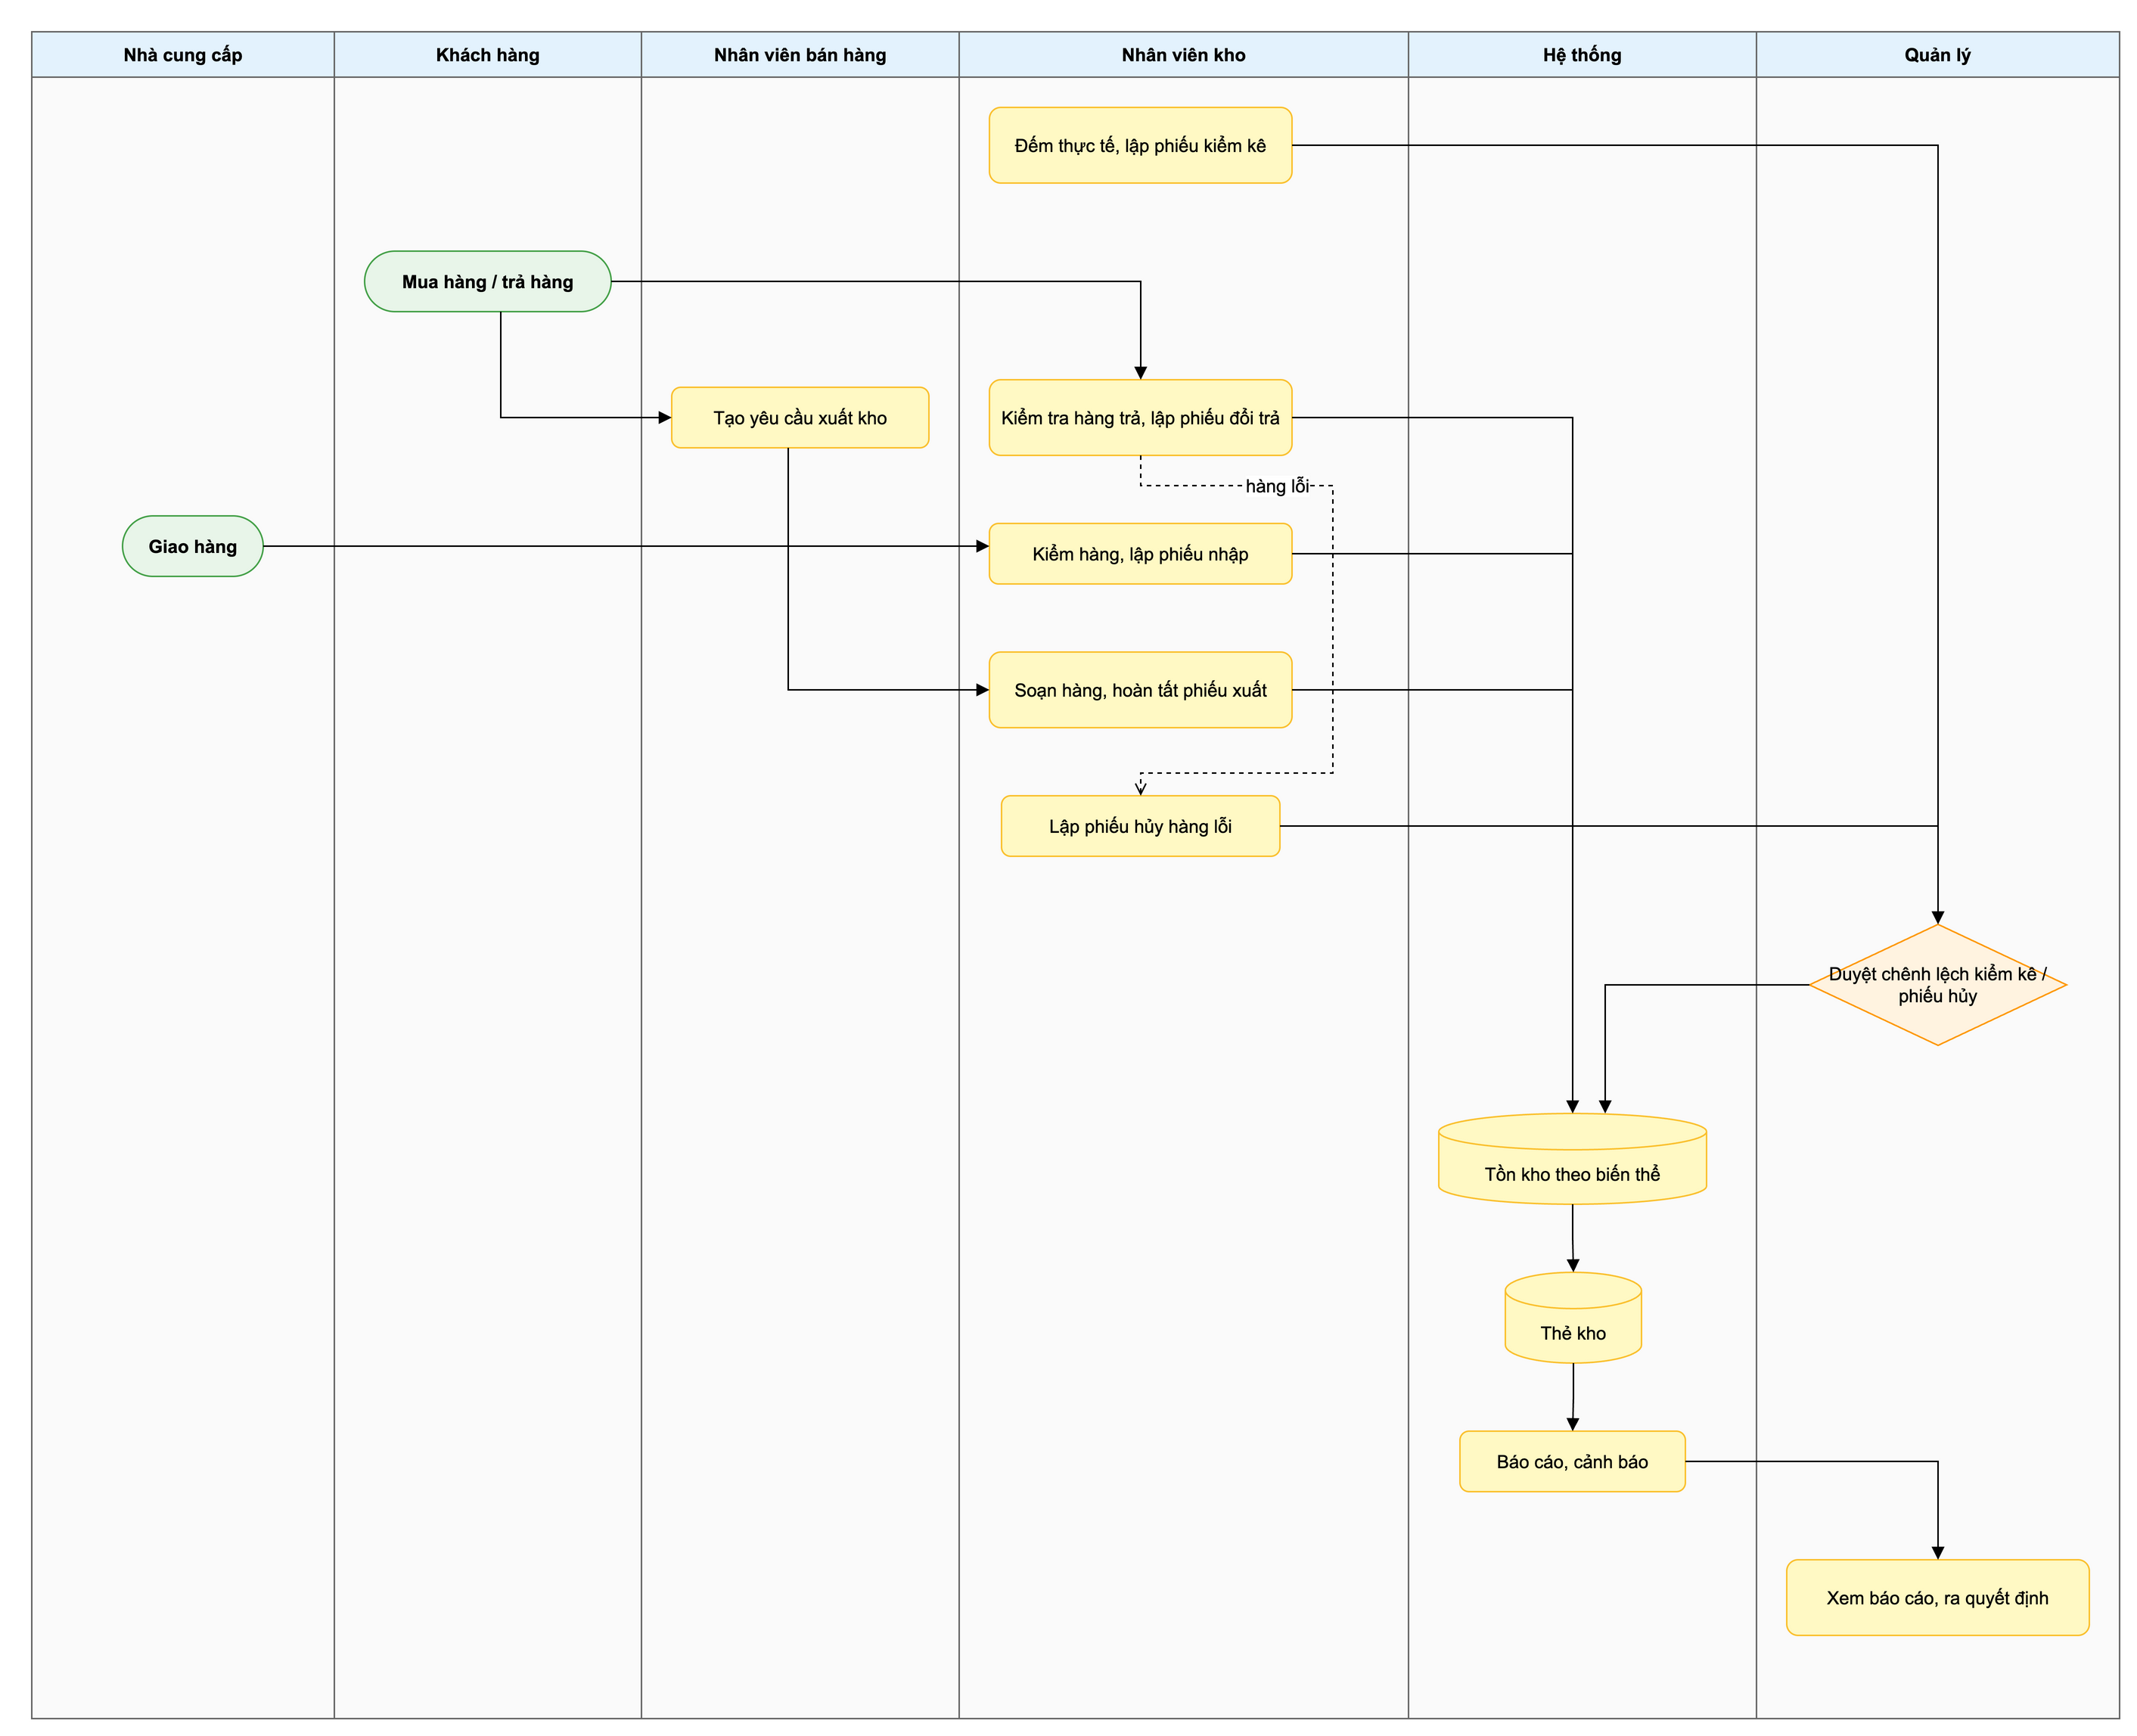
\includegraphics[width=0.86\textwidth]{assets/workflow.png}
\caption{Luồng nghiệp vụ tổng quát được trích từ báo cáo phân tích và thiết kế}
\label{fig:workflow}
\end{figure}

\section{Tác nhân}

\begin{table}[H]
\centering
\caption{Tác nhân trực tiếp của hệ thống}
\begin{tabularx}{\textwidth}{L{3.5cm}Y}
\toprule
\tablehead{Tác nhân} & \tablehead{Vai trò}\\
\midrule
Người dùng & Tác nhân trừu tượng đại diện cho người có tài khoản; đăng nhập và đổi mật khẩu.\\
Quản lý & Quản lý tài khoản, danh mục, nhà cung cấp, kho; duyệt kiểm kê, điều chỉnh, hủy hàng và xem báo cáo.\\
Nhân viên kho & Lập, hoàn tất phiếu nhập, xuất, chuyển, đổi trả, hủy; thực hiện kiểm kê và tra cứu tồn.\\
Nhân viên bán hàng & Tạo yêu cầu xuất kho cho đơn bán và tra cứu tồn để tư vấn khách.\\
\bottomrule
\end{tabularx}
\end{table}

\chapter{Phân tích yêu cầu}

\section{Yêu cầu chức năng}

Hồ sơ phân tích mã hóa 19 yêu cầu chức năng từ FR-01 đến FR-19 và truy vết mỗi yêu cầu tới một use case. Các yêu cầu được tổ chức thành bốn gói như Bảng~\ref{tab:packages}.

\begin{table}[H]
\centering
\caption{Bốn gói chức năng của hệ thống}
\label{tab:packages}
\begin{tabularx}{\textwidth}{L{3.2cm}C{1.2cm}Y}
\toprule
\tablehead{Gói} & \tablehead{Số UC} & \tablehead{Nội dung}\\
\midrule
Quản trị hệ thống & 2 & Đăng nhập; quản lý tài khoản, vai trò và kho phụ trách.\\
Quản lý danh mục & 5 & Sản phẩm; biến thể; loại, màu, kích thước; nhà cung cấp; kho và vị trí.\\
Nghiệp vụ kho & 8 & Nhập, yêu cầu xuất, xuất, chuyển, kiểm kê, duyệt điều chỉnh, đổi trả và hủy.\\
Tồn kho và báo cáo & 4 & Tra cứu tồn; cảnh báo tồn thấp; báo cáo kho; truy xuất biến động.\\
\midrule
\textbf{Tổng} & \textbf{19} & \textbf{19 yêu cầu chức năng được phủ bởi 19 use case.}\\
\bottomrule
\end{tabularx}
\end{table}

\begin{longtable}{L{1.35cm}L{6.0cm}L{7.0cm}}
\caption{Danh sách 19 yêu cầu chức năng}\label{tab:functional}\\
\toprule
\tablehead{Mã} & \tablehead{Yêu cầu chức năng} & \tablehead{Use case}\\
\midrule
\endfirsthead
\toprule
\tablehead{Mã} & \tablehead{Yêu cầu chức năng} & \tablehead{Use case}\\
\midrule
\endhead
FR-01 & Đăng nhập, đăng xuất và đổi mật khẩu. & UC-1.1\\
FR-02 & Quản lý tài khoản, gán vai trò và kho phụ trách, khóa tài khoản. & UC-1.2\\
FR-03 & Thêm, sửa, ngừng bán, tìm kiếm và lọc sản phẩm. & UC-2.1\\
FR-04 & Quản lý biến thể theo màu và size, sinh SKU, khai báo giá và tồn tối thiểu. & UC-2.2\\
FR-05 & Quản lý loại sản phẩm, màu sắc và kích thước. & UC-2.3\\
FR-06 & Quản lý nhà cung cấp và trạng thái hợp tác. & UC-2.4\\
FR-07 & Quản lý kho và vị trí lưu trữ. & UC-2.5\\
FR-08 & Lập phiếu nhập; hoàn tất thì cộng tồn và ghi thẻ kho. & UC-3.1\\
FR-09 & Tạo yêu cầu xuất kèm mã đơn hàng và xem tồn khả dụng. & UC-3.2\\
FR-10 & Xử lý xuất kho, kiểm tra đủ tồn, không cho tồn âm và ghi thẻ kho. & UC-3.3\\
FR-11 & Chuyển hàng qua hai bước xuất đi và xác nhận nhận hàng. & UC-3.4\\
FR-12 & Kiểm kê theo phạm vi và tự tính chênh lệch. & UC-3.5\\
FR-13 & Duyệt kiểm kê hoặc phiếu điều chỉnh và điều chỉnh theo chênh lệch. & UC-3.6\\
FR-14 & Tiếp nhận đổi trả, nhập hàng tốt, tách hàng lỗi, xuất hàng đổi và tính chênh lệch. & UC-3.7\\
FR-15 & Lập phiếu hủy hàng lỗi, hỏng; chỉ có hiệu lực sau khi duyệt. & UC-3.8\\
FR-16 & Tra cứu tồn theo kho, sản phẩm, màu, size, vị trí và trạng thái. & UC-4.1\\
FR-17 & Cảnh báo biến thể hết hàng hoặc sắp hết theo tồn tối thiểu. & UC-4.2\\
FR-18 & Lập sáu nhóm báo cáo kho và xuất định dạng Excel. & UC-4.3\\
FR-19 & Truy xuất lịch sử biến động theo thời gian, chứng từ, số lượng và người thực hiện. & UC-4.4\\
\bottomrule
\end{longtable}

\section{Yêu cầu phi chức năng}

\begin{longtable}{L{1.35cm}L{2.8cm}L{10.2cm}}
\caption{Danh sách 11 yêu cầu phi chức năng}\label{tab:nonfunctional}\\
\toprule
\tablehead{Mã} & \tablehead{Nhóm} & \tablehead{Tiêu chí}\\
\midrule
\endfirsthead
\toprule
\tablehead{Mã} & \tablehead{Nhóm} & \tablehead{Tiêu chí}\\
\midrule
\endhead
NFR-01 & Hiệu năng & Tra cứu tồn dưới 2 giây với 50.000 biến thể và 100 người dùng đồng thời.\\
NFR-02 & Hiệu năng & Báo cáo nhập - xuất - tồn một tháng cho toàn bộ kho dưới 10 giây.\\
NFR-03 & Toàn vẹn dữ liệu & Hoàn tất phiếu kho là một giao dịch nguyên tử: cập nhật tồn, ghi thẻ kho và đổi trạng thái cùng thành công hoặc cùng hủy.\\
NFR-04 & Toàn vẹn dữ liệu & Hai phiếu xuất đồng thời trên cùng biến thể không làm tồn âm; cập nhật có khóa dòng tồn kho.\\
NFR-05 & Truy vết & Thẻ kho chỉ được thêm, không sửa hoặc xóa, và được lưu tối thiểu 5 năm.\\
NFR-06 & Bảo mật & RBAC; mật khẩu băm bằng bcrypt; khóa tài khoản 15 phút sau 5 lần đăng nhập sai.\\
NFR-07 & Bảo mật & Toàn bộ truy cập qua HTTPS; phiên hết hạn sau 30 phút không thao tác.\\
NFR-08 & Khả dụng & Sẵn sàng 99\% trong giờ làm việc từ 7h đến 22h; sao lưu hằng ngày và khôi phục trong 4 giờ.\\
NFR-09 & Dễ sử dụng & Giao diện tiếng Việt, hỗ trợ máy quét mã vạch và dùng được trên máy tính bảng 10 inch.\\
NFR-10 & Tương thích & Chạy trên Chrome, Edge trong hai năm gần nhất và xuất báo cáo .xlsx.\\
NFR-11 & Bảo trì & Kiến trúc phân lớp, tách hệ thống con theo nghiệp vụ để có thể mở rộng tích hợp bán hàng.\\
\bottomrule
\end{longtable}

\section{Use case và phân quyền}

\begin{table}[H]
\centering
\caption{Phân nhóm 19 use case}
\small
\begin{tabularx}{\textwidth}{L{3.0cm}L{3.0cm}Y}
\toprule
\tablehead{Gói} & \tablehead{Mã use case} & \tablehead{Tên use case}\\
\midrule
Quản trị hệ thống & UC-1.1 - UC-1.2 & Đăng nhập; Quản lý tài khoản.\\
Quản lý danh mục & UC-2.1 - UC-2.5 & Quản lý sản phẩm; biến thể; loại, màu, kích thước; nhà cung cấp; kho và vị trí.\\
Nghiệp vụ kho & UC-3.1 - UC-3.8 & Nhập; tạo yêu cầu xuất; xuất; chuyển kho; kiểm kê; duyệt điều chỉnh; đổi trả; hủy hàng.\\
Tồn kho và báo cáo & UC-4.1 - UC-4.4 & Tra cứu tồn; cảnh báo tồn thấp; lập báo cáo; truy xuất biến động.\\
\bottomrule
\end{tabularx}
\end{table}

\begin{table}[H]
\centering
\caption{Ma trận phân quyền rút gọn}
\small
\begin{tabularx}{\textwidth}{Y C{2.1cm} C{2.1cm} C{2.3cm}}
\toprule
\tablehead{Chức năng} & \tablehead{Quản lý} & \tablehead{Nhân viên kho} & \tablehead{Nhân viên bán hàng}\\
\midrule
Đăng nhập & X & X & X\\
Quản lý tài khoản & X &  & \\
Quản lý danh mục & X & Chỉ xem & Chỉ xem sản phẩm\\
Nhập kho & Xem & X & \\
Tạo yêu cầu xuất & Xem &  & X\\
Xuất kho, chuyển kho, kiểm kê, đổi trả & Xem & X & \\
Duyệt điều chỉnh tồn & X &  & \\
Hủy hàng & X (duyệt) & X & \\
Tra cứu tồn & X & X & X\\
Cảnh báo và truy xuất thẻ kho & X & X & \\
Lập báo cáo & X &  & \\
\bottomrule
\end{tabularx}
\end{table}

\section{Các use case trọng tâm}

\subsection{Nhập kho}
Nhân viên kho lập phiếu theo nhà cung cấp, quét hoặc nhập các dòng SKU, kiểm tra dữ liệu và hoàn tất phiếu. Khi hoàn tất, hệ thống cộng tồn cho từng cặp kho - biến thể, ghi thẻ kho và đổi trạng thái phiếu trong cùng giao dịch.

\subsection{Xuất kho}
Nhân viên bán hàng tạo yêu cầu xuất kèm mã đơn hàng. Nhân viên kho xử lý phiếu, kiểm tra tồn khả dụng và chỉ hoàn tất khi đủ tồn. Nếu thiếu, phiếu bị từ chối theo luồng ngoại lệ; cơ chế khóa dòng bảo đảm hai yêu cầu đồng thời không làm tồn âm.

\subsection{Duyệt điều chỉnh tồn kho}
Phiếu kiểm kê ghi số thực tế và chênh lệch bằng thực tế trừ hệ thống. Quản lý duyệt hoặc từ chối. Khi duyệt, hệ thống điều chỉnh theo giá trị chênh lệch thay vì ghi đè số tồn, nhờ đó các biến động phát sinh sau thời điểm kiểm kê không bị mất.

\subsection{Đổi trả hàng}
Hàng trả được phân loại theo tình trạng. Hàng còn tốt nhập lại kho bán; hàng lỗi, hỏng chuyển vào kho hàng lỗi. Nếu có hàng đổi sang, hệ thống xuất biến thể mới và tính tiền chênh lệch theo giá bán của hai nhóm hàng.

\chapter{Phân tích và thiết kế hệ thống}

\section{Mô hình lĩnh vực}

Ba quyết định mô hình hóa chính được nêu trong báo cáo phân tích là:
\begin{itemize}
\item Tách \textit{SanPham} là mẫu sản phẩm và \textit{BienTheSanPham} là tổ hợp màu, size. Tồn kho gắn với biến thể.
\item \textit{TonKho} là lớp liên kết giữa \textit{Kho} và \textit{BienTheSanPham}; mỗi cặp kho - biến thể có một bản ghi tồn.
\item Sáu loại phiếu nhập, xuất, chuyển kho, điều chỉnh, hủy và đổi trả được tổng quát hóa thành \textit{PhieuKho}. Khi hoàn tất, phiếu sinh các dòng \textit{LichSuBienDong}; phiếu kiểm kê được mô hình hóa riêng.
\end{itemize}

\begin{figure}[H]
\centering
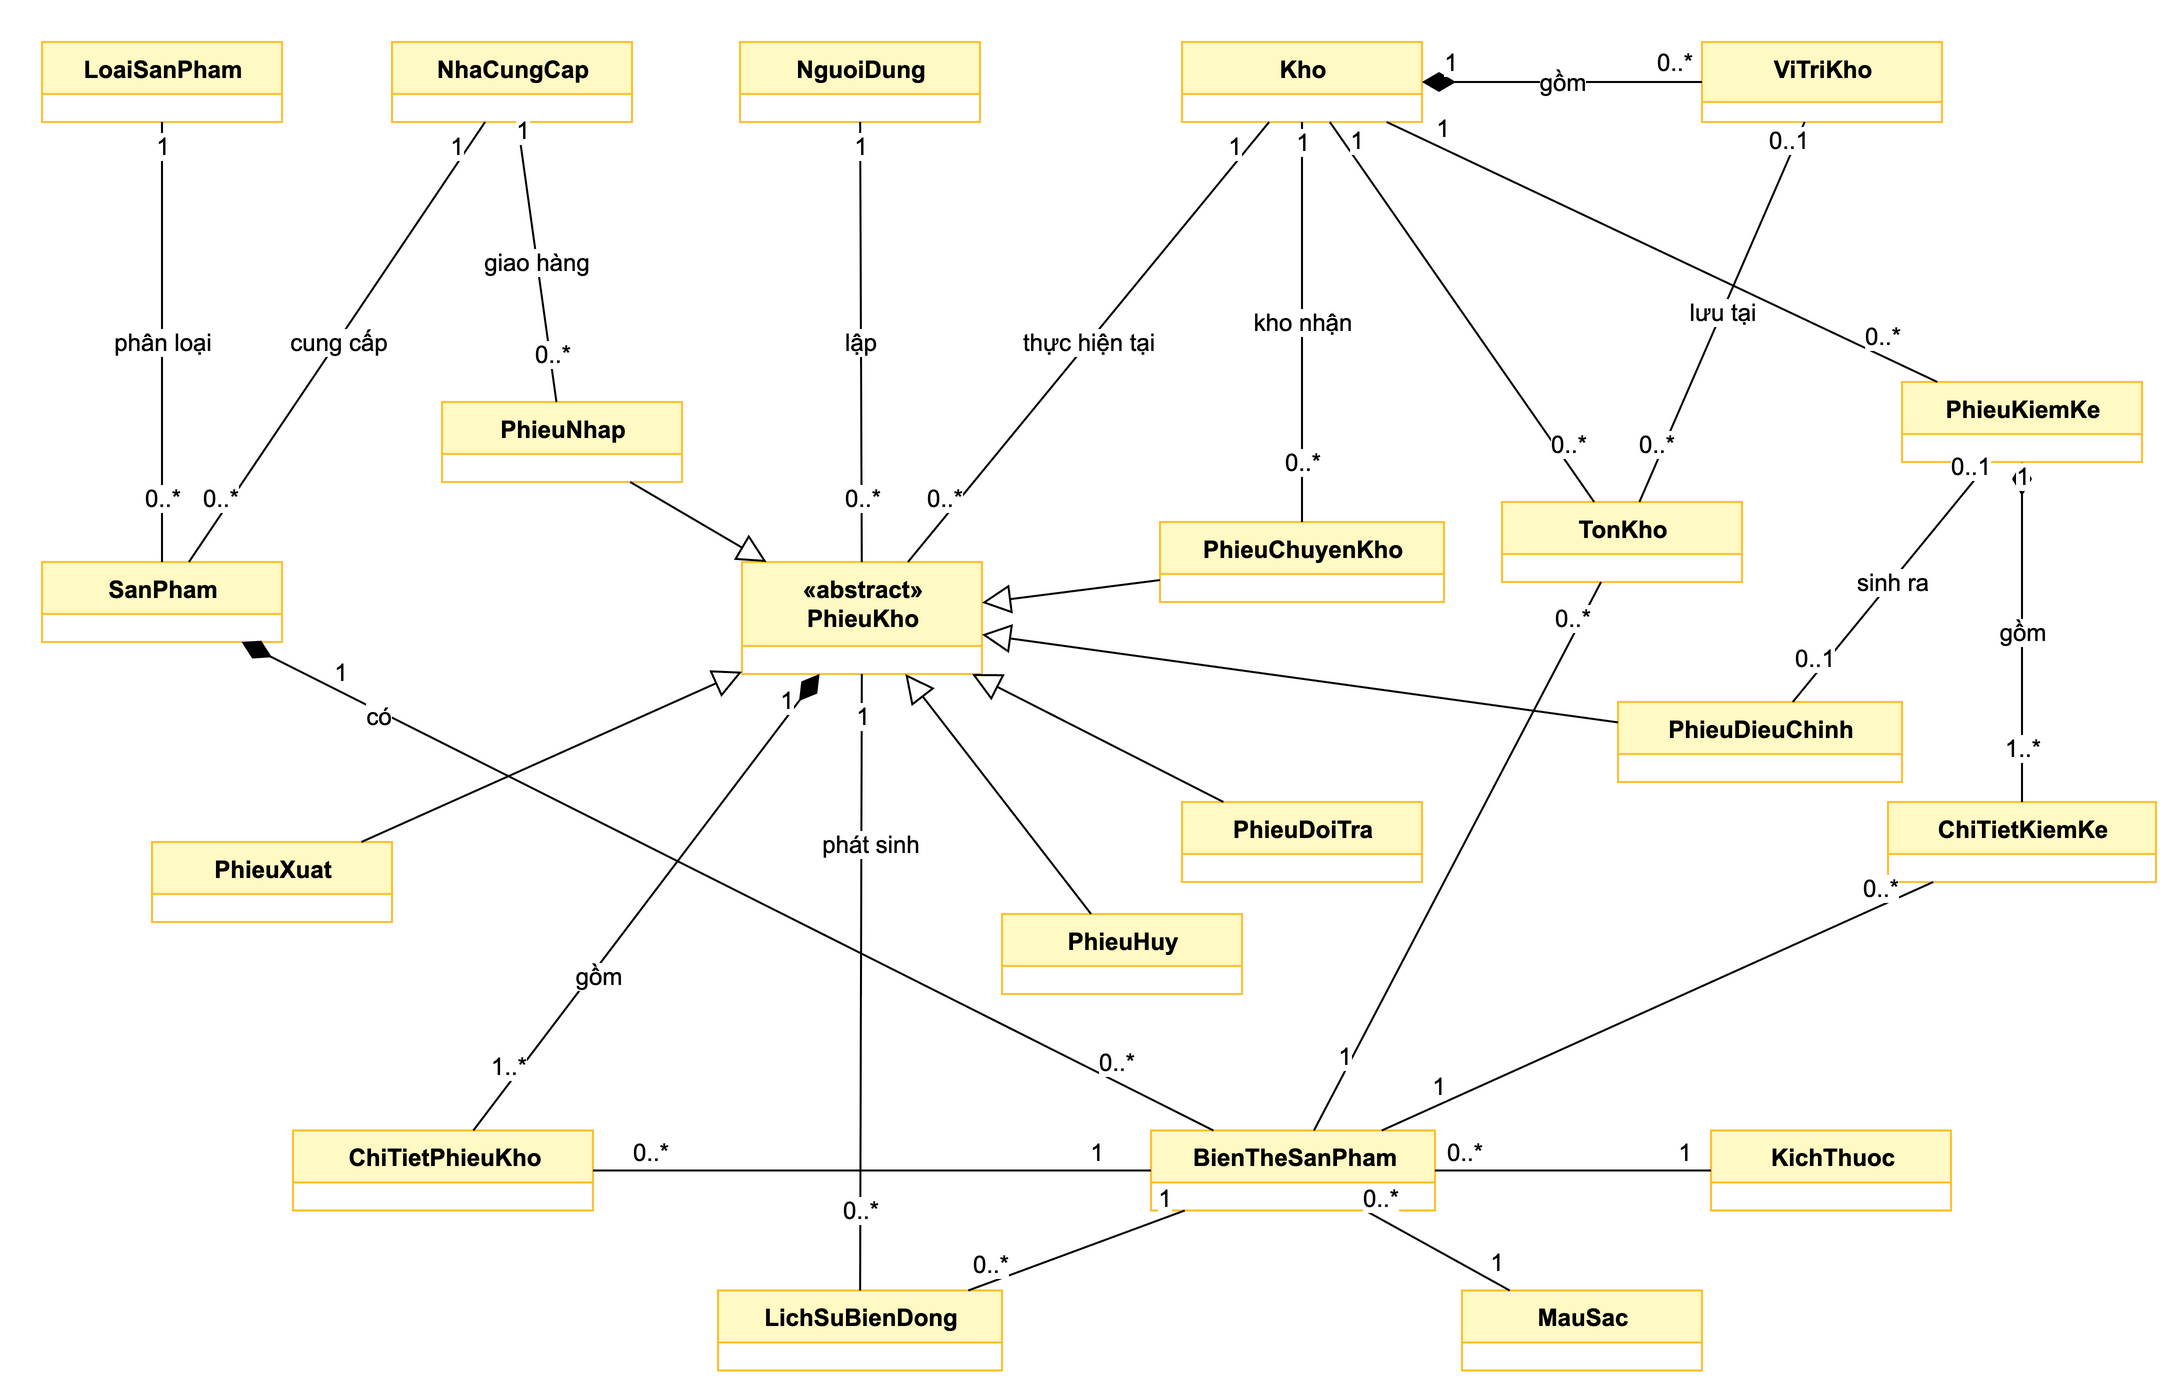
\includegraphics[width=0.92\textwidth]{assets/domain.png}
\caption{Mô hình lĩnh vực của hệ thống quản lý kho thời trang}
\label{fig:domain}
\end{figure}

\section{Phân tích hành vi}

Bốn use case trọng tâm được phân tích theo mẫu BCE gồm lớp biên, lớp điều khiển và lớp thực thể. \textit{TonKho} và \textit{LichSuBienDong} xuất hiện trong cả bốn nhóm use case trọng tâm, thể hiện vai trò lõi của chúng.

Các biểu đồ tuần tự mô tả việc cập nhật tồn và ghi thẻ kho trong giao dịch khi nhập kho, rẽ nhánh đủ hoặc thiếu tồn khi xuất kho, điều chỉnh theo chênh lệch khi duyệt kiểm kê và phân loại hàng trả theo tình trạng. Các biểu đồ hoạt động mô tả luồng yêu cầu - xuất kho, kiểm kê - điều chỉnh và đổi trả - hủy hàng. Biểu đồ trạng thái của \textit{PhieuKho} chỉ cho phép thay đổi tồn ở chuyển trạng thái đi vào Hoàn thành hoặc Đang vận chuyển; trong trạng thái đang kiểm kê, các biến thể thuộc phạm vi được tạm khóa nhập và xuất.

\section{Kiến trúc và công nghệ}

Hệ thống được thiết kế theo mô hình ứng dụng web ba tầng. Tầng trình bày là SPA trên trình duyệt máy tính và máy tính bảng, máy quét mã vạch hoạt động như bàn phím. Tầng ứng dụng cung cấp REST API và tổ chức theo BCE. Tầng dữ liệu là hệ quản trị cơ sở dữ liệu quan hệ.

\begin{table}[H]
\centering
\caption{Công nghệ dự kiến sử dụng}
\small
\begin{tabularx}{\textwidth}{L{2.7cm}L{5.2cm}Y}
\toprule
\tablehead{Tầng} & \tablehead{Công nghệ} & \tablehead{Vai trò}\\
\midrule
Trình bày & ReactJS, TypeScript & Ứng dụng web một trang, responsive cho máy tính bảng.\\
Ứng dụng & Java 21, Spring Boot 3, Spring Security & REST API, JWT, RBAC và quản lý giao dịch.\\
Truy cập dữ liệu & Spring Data JPA (Hibernate) & Ánh xạ lớp thực thể và khóa bi quan khi cập nhật tồn.\\
Dữ liệu & PostgreSQL 16 & Lưu trữ nghiệp vụ và ràng buộc toàn vẹn.\\
Báo cáo & Apache POI & Sinh tệp Excel .xlsx.\\
Hạ tầng & Nginx, Docker & Reverse proxy HTTPS và đóng gói triển khai.\\
\bottomrule
\end{tabularx}
\end{table}

\section{Các hệ thống con}

\begin{table}[H]
\centering
\caption{Sáu hệ thống con}
\small
\begin{tabularx}{\textwidth}{L{3.2cm}L{5.0cm}Y}
\toprule
\tablehead{Hệ thống con} & \tablehead{Trách nhiệm} & \tablehead{Use case hoặc lớp chính}\\
\midrule
Quản trị và bảo mật & Xác thực, phiên, tài khoản và phân quyền. & UC-1.1, UC-1.2; NguoiDung.\\
Danh mục hàng hóa & Sản phẩm, biến thể, loại, màu, size, NCC, kho, vị trí. & UC-2.1 đến UC-2.5.\\
Nghiệp vụ kho & Vòng đời phiếu nhập, xuất, chuyển, đổi trả và hủy. & UC-3.1 đến UC-3.4, UC-3.7, UC-3.8.\\
Kiểm kê & Phiếu kiểm kê, duyệt và sinh phiếu điều chỉnh. & UC-3.5, UC-3.6.\\
Tồn kho và thẻ kho & Cập nhật có khóa, ghi thẻ kho, tra cứu và cảnh báo. & UC-4.1, UC-4.2, UC-4.4.\\
Báo cáo & Tổng hợp số liệu và xuất Excel. & UC-4.3.\\
\bottomrule
\end{tabularx}
\end{table}

\begin{figure}[H]
\centering
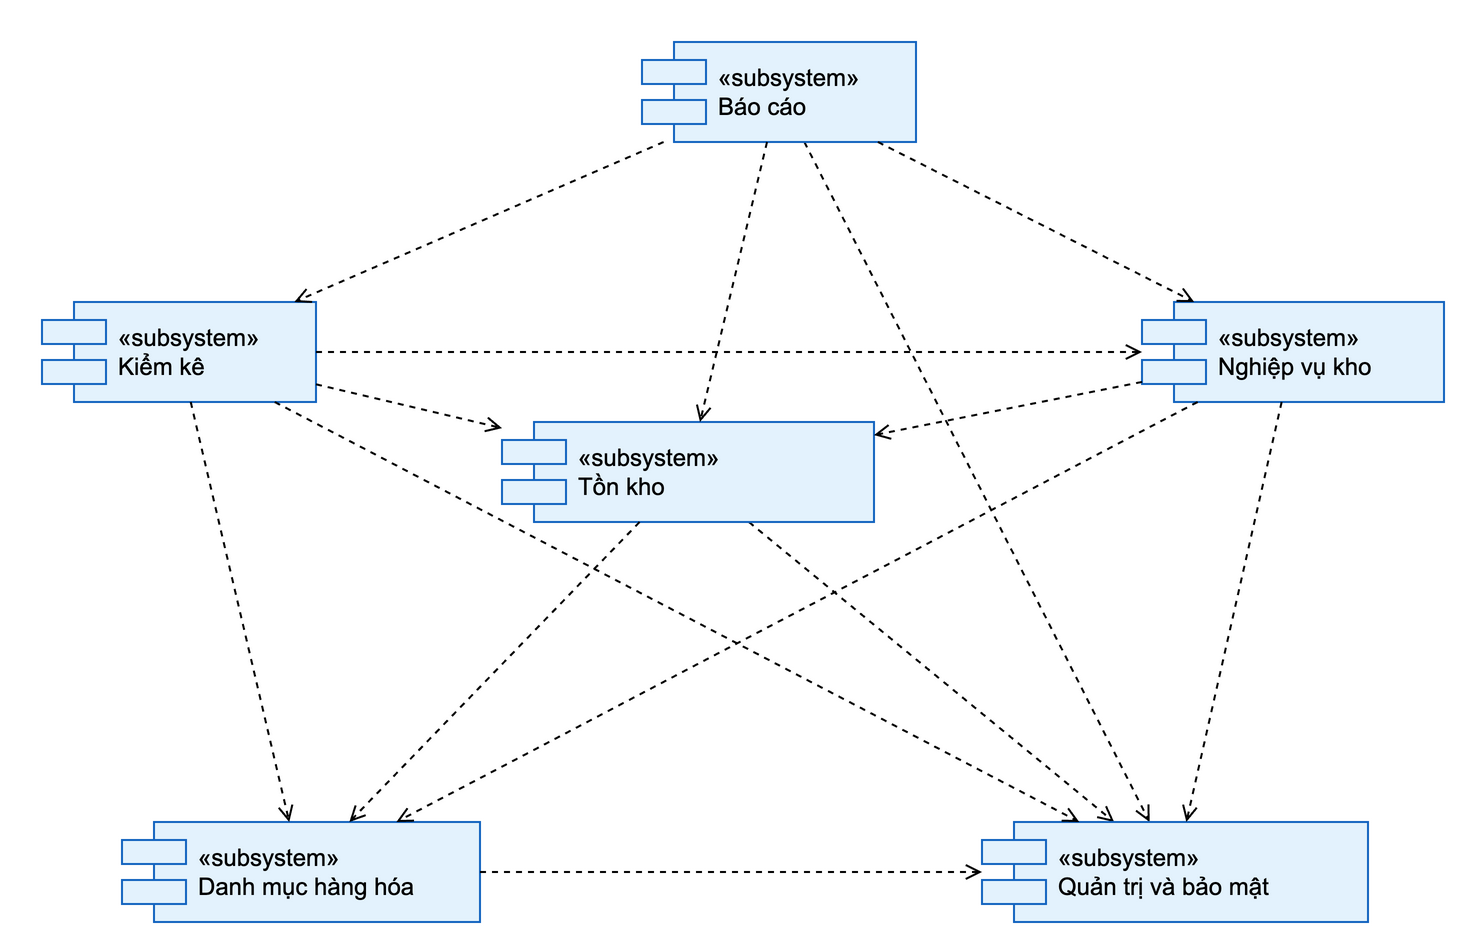
\includegraphics[width=0.84\textwidth]{assets/subsystems.png}
\caption{Quan hệ phụ thuộc giữa các hệ thống con}
\label{fig:subsystems}
\end{figure}

\section{Triển khai}

Thiết kế triển khai đề xuất máy chủ ứng dụng 4 vCPU, 8 GB RAM, Ubuntu 22.04 và Docker; máy chủ cơ sở dữ liệu 4 vCPU, 16 GB RAM, SSD 200 GB; lưu trữ sao lưu dạng object storage giữ 30 bản gần nhất; máy tính bảng 10 inch tại kho. Máy chủ cơ sở dữ liệu chỉ nhận kết nối từ máy chủ ứng dụng trong mạng riêng, còn truy cập bên ngoài đi qua cổng HTTPS.

\begin{figure}[H]
\centering
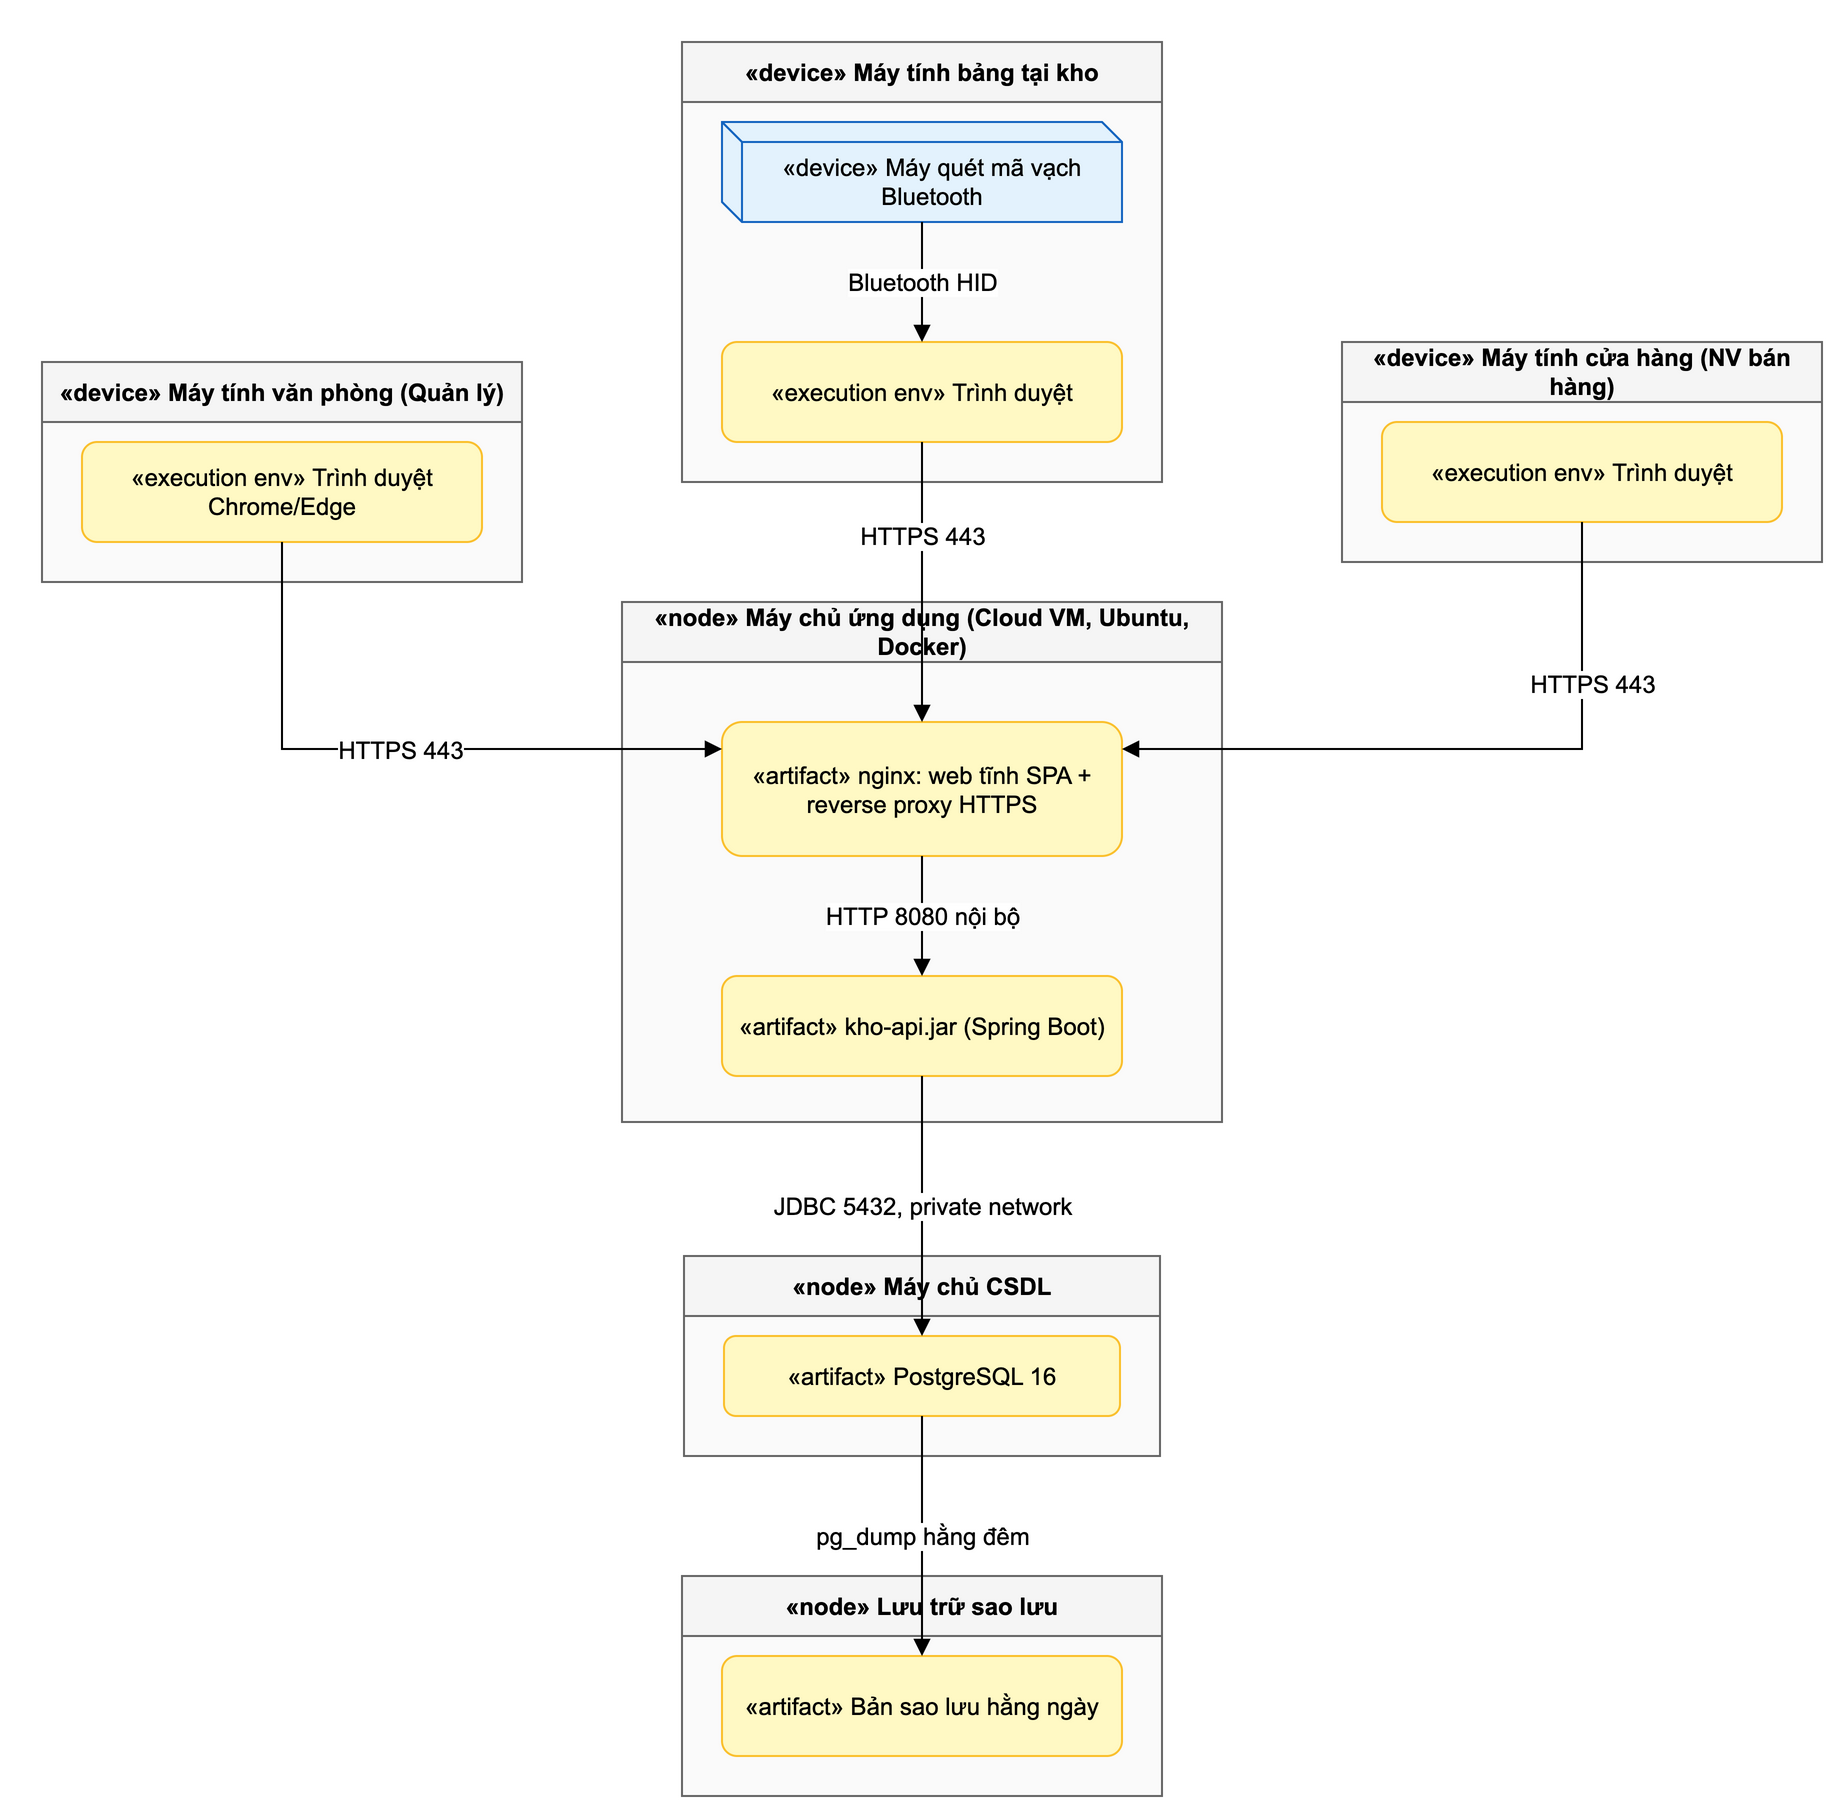
\includegraphics[width=0.82\textwidth]{assets/deployment.png}
\caption{Biểu đồ triển khai trong báo cáo phân tích và thiết kế}
\label{fig:deployment}
\end{figure}

\section{Cơ sở dữ liệu}

Thiết kế ánh xạ lớp thực thể sang 15 bảng quan hệ. Thuộc tính camelCase đổi sang tên cột snake\_case. Cây kế thừa \textit{PhieuKho} dùng chiến lược một bảng với cột phân biệt loại phiếu. Tiền tệ dùng \texttt{numeric(12,0)} vì đơn vị tính là đồng.

\begin{table}[H]
\centering
\caption{Các nhóm bảng trong thiết kế dữ liệu}
\small
\begin{tabularx}{\textwidth}{L{4.3cm}Y}
\toprule
\tablehead{Nhóm} & \tablehead{Bảng hoặc lớp thực thể}\\
\midrule
Người dùng và danh mục & \texttt{nguoi\_dung}, \texttt{loai\_san\_pham}, \texttt{mau\_sac}, \texttt{kich\_thuoc}, \texttt{san\_pham}, \texttt{bien\_the\_san\_pham}, \texttt{nha\_cung\_cap}.\\
Kho và vị trí & \texttt{kho}, \texttt{vi\_tri\_kho}, \texttt{ton\_kho}.\\
Chứng từ & Cây \texttt{phieu\_kho} và \texttt{chi\_tiet\_phieu\_kho}.\\
Kiểm kê & \texttt{phieu\_kiem\_ke}, \texttt{chi\_tiet\_kiem\_ke}.\\
Truy vết & \texttt{lich\_su\_bien\_dong}.\\
\bottomrule
\end{tabularx}
\end{table}

Các ràng buộc quan trọng gồm \texttt{CHECK so\_luong >= 0} trên tồn kho, \texttt{UNIQUE (kho, bien\_the)} và chỉ mục theo biến thể, kho, thời gian trên lịch sử biến động. Thẻ kho chỉ cho phép thêm và truy vấn, không có thao tác sửa hoặc xóa.

\begin{figure}[H]
\centering
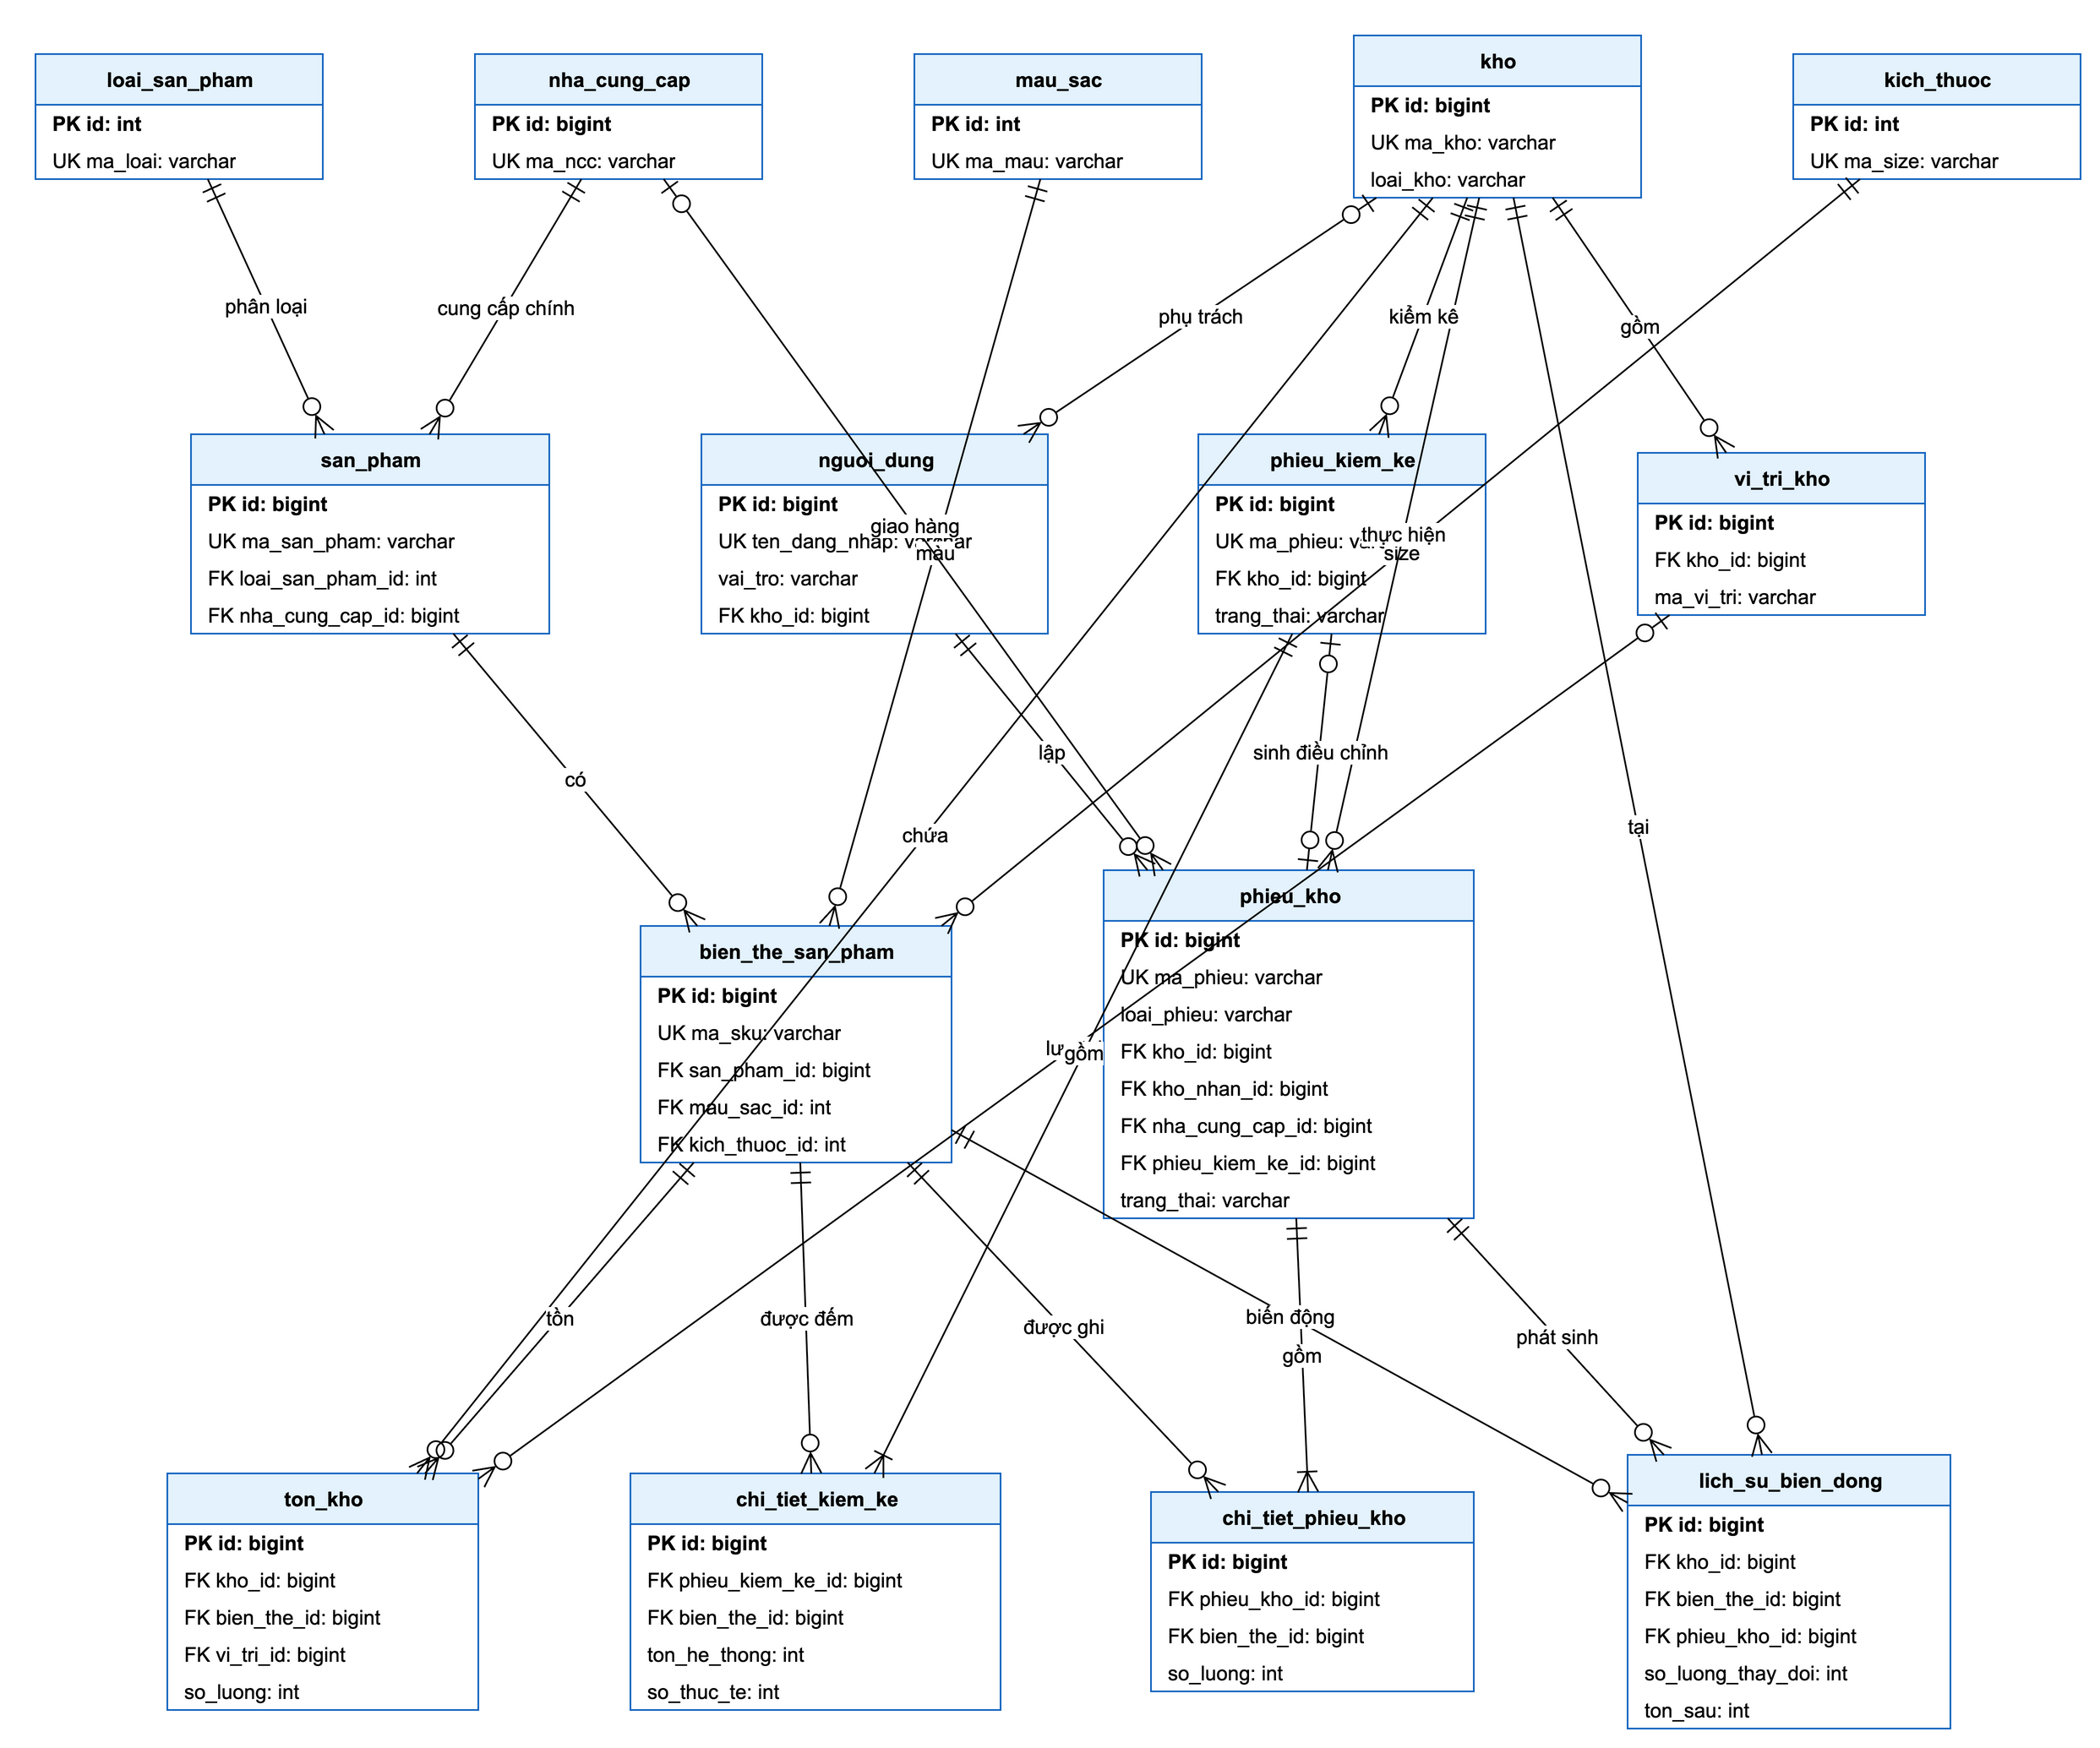
\includegraphics[width=\textwidth,height=0.68\textheight,keepaspectratio]{assets/database.png}
\caption{Lược đồ cơ sở dữ liệu}
\label{fig:database}
\end{figure}

\section{Thiết kế giao diện}

Giao diện dành cho màn hình từ 10 inch, gồm menu trái hiển thị theo quyền, thanh tiêu đề có ô tìm SKU và vùng nội dung. Ô nhập SKU nhận dữ liệu từ máy quét mã vạch; sau khi quét, con trỏ chuyển sang ô số lượng.

\begin{longtable}{L{1.2cm}L{4.2cm}L{2.4cm}L{6.0cm}}
\caption{Danh sách 10 màn hình}\label{tab:screens}\\
\toprule
\tablehead{Mã} & \tablehead{Màn hình} & \tablehead{Use case} & \tablehead{Mục đích}\\
\midrule
\endfirsthead
\toprule
\tablehead{Mã} & \tablehead{Màn hình} & \tablehead{Use case} & \tablehead{Mục đích}\\
\midrule
\endhead
MH-01 & Đăng nhập & UC-1.1 & Xác thực người dùng.\\
MH-02 & Tổng quan & UC-4.2 & Cảnh báo tồn thấp và phiếu chờ xử lý.\\
MH-03 & Sản phẩm và biến thể & UC-2.1, UC-2.2 & Quản lý mẫu và sinh ma trận màu x size.\\
MH-04 & Lập phiếu nhập kho & UC-3.1 & Quét hàng nhập và hoàn tất phiếu.\\
MH-05 & Xử lý phiếu xuất & UC-3.2, UC-3.3 & Danh sách yêu cầu và soạn hàng xuất.\\
MH-06 & Kiểm kê & UC-3.5 & Nhập số thực tế theo phạm vi.\\
MH-07 & Duyệt kiểm kê & UC-3.6 & Xem chênh lệch và duyệt điều chỉnh.\\
MH-08 & Đổi trả hàng & UC-3.7, UC-3.8 & Ghi nhận hàng trả và hàng đổi.\\
MH-09 & Tra cứu tồn kho và thẻ kho & UC-4.1, UC-4.4 & Lọc tồn và xem lịch sử.\\
MH-10 & Báo cáo & UC-4.3 & Lọc báo cáo và xuất Excel.\\
\bottomrule
\end{longtable}

MH-04 cho phép quét liên tiếp các SKU, quét lại SKU đã có thì tăng số lượng, chỉ cho số lượng nguyên dương và vô hiệu hóa nút Hoàn tất khi chưa có dòng hàng. MH-07 mặc định hiển thị dòng có chênh lệch, tổng hợp thiếu/thừa và bắt buộc nhập lý do khi duyệt hoặc từ chối. MH-09 lọc theo kho, loại, màu, size, trạng thái, phân trang 50 dòng và mở thẻ kho ngay dưới dòng được chọn.

\begin{figure}[H]
\centering
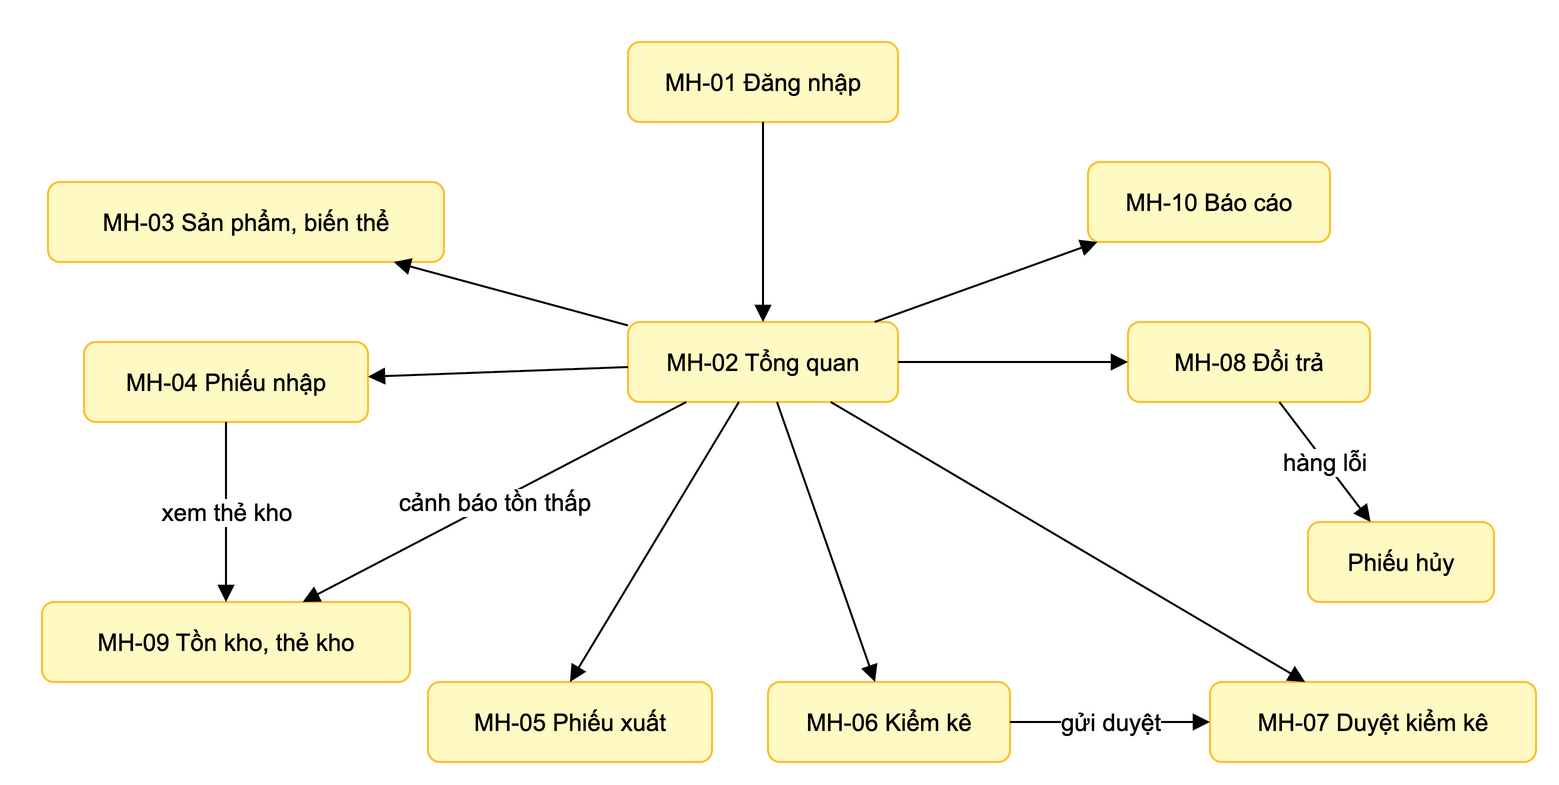
\includegraphics[width=0.84\textwidth]{assets/screenflow.png}
\caption{Luồng chuyển giữa các màn hình chính}
\label{fig:screenflow}
\end{figure}

\begin{figure}[H]
\centering
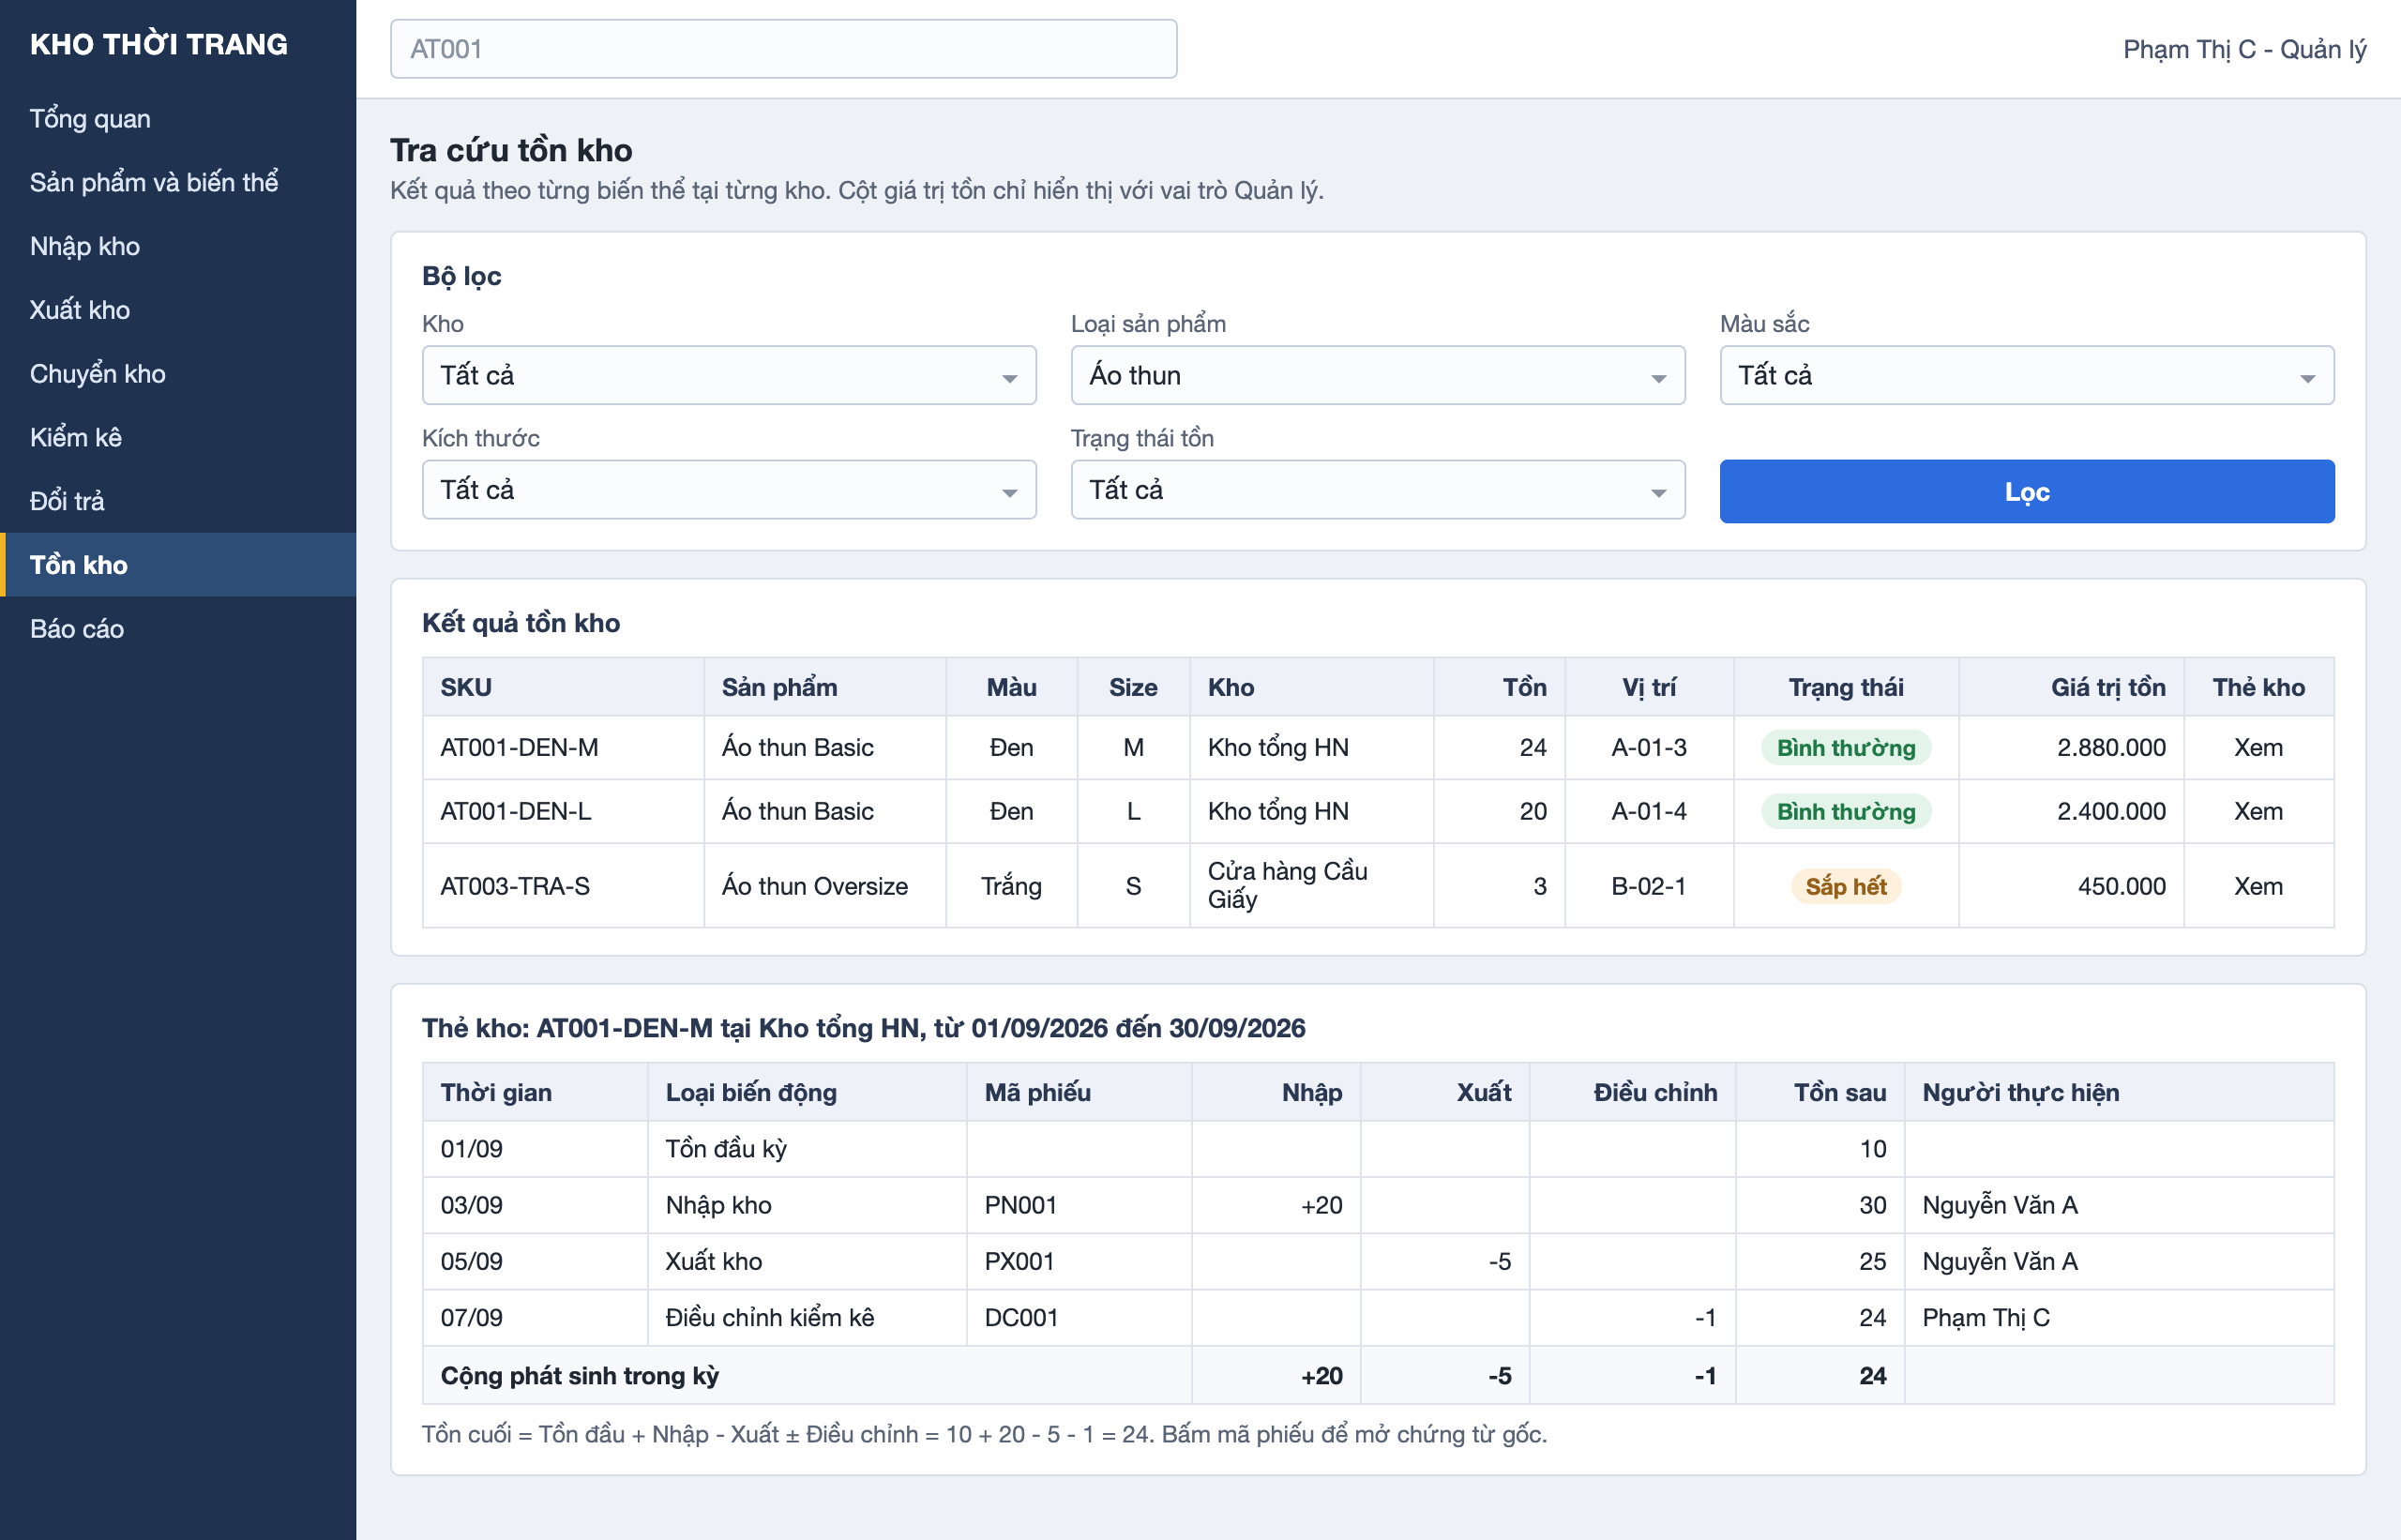
\includegraphics[width=\textwidth,height=0.52\textheight,keepaspectratio]{assets/ui_inventory.png}
\caption{Phác thảo màn hình tra cứu tồn kho và thẻ kho}
\label{fig:uiinventory}
\end{figure}

\chapter{Kế hoạch công việc và tiến độ}

\section{Cấu trúc phân rã công việc}

WBS hiện hành gồm 52 task chia thành sáu giai đoạn. Các task dùng ước lượng PERT theo công thức
\[
\mathrm{EST}_{\mathrm{PERT}}=\frac{\mathrm{MO}+4\mathrm{ML}+\mathrm{MP}}{6},
\qquad
\mathrm{EST}_{\mathrm{chốt}}=\mathrm{EST}_{\mathrm{PERT}}(1+10\%).
\]

\begin{table}[H]
\centering
\caption{Sáu giai đoạn và sản phẩm chính}
\small
\begin{tabularx}{\textwidth}{L{0.9cm}L{3.0cm}L{3.0cm}L{1.2cm}Y}
\toprule
\tablehead{Mã} & \tablehead{Giai đoạn} & \tablehead{Thời gian} & \tablehead{Task} & \tablehead{Sản phẩm và nội dung}\\
\midrule
A & Khảo sát và yêu cầu & 01/09/2026 - 25/09/2026 & 1-8 & Báo cáo khảo sát, đặc tả yêu cầu, mục tiêu, phạm vi và quy tắc nghiệp vụ.\\
B & Phân tích và thiết kế hệ thống & 26/09/2026 - 20/11/2026 & 9-17 & Mô hình tác nhân, use case, lớp, tuần tự, hoạt động, trạng thái và kiến trúc.\\
C & Thiết kế CSDL và giao diện & 21/11/2026 - 25/12/2026 & 18-25 & Lược đồ 15 bảng, từ điển dữ liệu, script CSDL và thiết kế 10 màn hình.\\
D & Xây dựng chương trình & 26/12/2026 - 15/02/2027 & 26-39 & Mã nguồn, dịch vụ tồn kho, nghiệp vụ kho, báo cáo, giao diện web.\\
E & Tích hợp và kiểm thử & 16/02/2027 - 15/03/2027 & 40-47 & Tích hợp module, test chức năng, đồng thời, hiệu năng, bảo mật, UAT và sửa lỗi.\\
F & Triển khai và bàn giao & 16/03/2027 - 31/03/2027 & 48-52 & Môi trường triển khai, chuyển đổi dữ liệu, tài liệu, báo cáo nghiệm thu và đào tạo.\\
\bottomrule
\end{tabularx}
\end{table}

\section{Khối lượng theo giai đoạn}

\begin{table}[H]
\centering
\caption{Khối lượng chốt theo giai đoạn}
\begin{tabularx}{\textwidth}{L{2cm}C{2.2cm}Y}
\toprule
\tablehead{Giai đoạn} & \tablehead{Manday chốt} & \tablehead{Diễn giải}\\
\midrule
A & 27,13 & Khảo sát, hợp nhất hiện trạng và đặc tả yêu cầu.\\
B & 41,07 & Phân tích, mô hình hóa và thiết kế kiến trúc.\\
C & 29,88 & CSDL, script dữ liệu và giao diện.\\
D & 69,30 & Xây dựng các module và 10 màn hình.\\
E & 41,07 & Tích hợp, kiểm thử, UAT và sửa lỗi.\\
F & 13,38 & Triển khai, tài liệu, nghiệm thu và đào tạo.\\
\midrule
\textbf{Tổng} & \textbf{221,83} & Tổng khối lượng trong bảng tổng hợp WBS.\\
\bottomrule
\end{tabularx}
\end{table}

\section{Phân bổ khối lượng theo thành viên}

\begin{table}[H]
\centering
\caption{Tổng manday chốt theo thành viên}
\begin{tabularx}{\textwidth}{L{5.0cm}C{2.6cm}Y}
\toprule
\tablehead{Thành viên} & \tablehead{Manday} & \tablehead{Vai trò nổi bật trong WBS}\\
\midrule
Bùi Tuấn Anh & 43,27 & Chủ nhiệm, khảo sát, yêu cầu, báo cáo và UAT.\\
Bùi Quốc Luýt & 48,95 & Trưởng nhóm kỹ thuật, kiến trúc, dịch vụ tồn kho, xuất kho và sửa lỗi.\\
Vũ Quang Minh & 41,98 & Back-end, script CSDL, danh mục, nhập kho, chuyển kho và kiểm thử.\\
Bạch Minh Quang & 44,00 & UI/UX, front-end, tra cứu, kiểm thử giao diện và đào tạo.\\
Phạm Đoàn Bảo Thiên & 43,63 & Đặc tả use case, CSDL, kiểm kê, đổi trả, kiểm thử và tài liệu.\\
\midrule
\textbf{Tổng} & \textbf{221,83} & \\
\bottomrule
\end{tabularx}
\end{table}

\section{Các mốc kiểm soát}

\begin{table}[H]
\centering
\caption{Mốc kiểm soát chất lượng và điều kiện chuyển giai đoạn}
\small
\begin{tabularx}{\textwidth}{L{2.8cm}L{2.0cm}Y L{3.0cm}}
\toprule
\tablehead{Mốc} & \tablehead{Thời điểm} & \tablehead{Điều kiện đạt} & \tablehead{Người phê duyệt}\\
\midrule
M1 - Chốt yêu cầu & 25/09/2026 & Đặc tả yêu cầu được doanh nghiệp xác nhận. & Bùi Tuấn Anh và đại diện doanh nghiệp.\\
M2 - Chốt phân tích thiết kế & 20/11/2026 & UML và kiến trúc qua rà soát, không còn ý kiến nghiêm trọng. & Bùi Tuấn Anh, Bùi Quốc Luýt.\\
M3 - Chốt CSDL và giao diện & 25/12/2026 & Lược đồ và script chạy được; prototype 10 màn hình được duyệt. & Bùi Tuấn Anh và đại diện doanh nghiệp.\\
M4 - Hoàn thành lập trình & 15/02/2027 & Đủ chức năng theo WBS, unit test đạt yêu cầu, không có lỗi Blocker/Critical từ phân tích tĩnh. & Bùi Quốc Luýt.\\
M5 - Hoàn thành kiểm thử & 15/03/2027 & Ít nhất 95\% test case đạt, không còn lỗi Blocker/Critical, đạt NFR-01 và NFR-02. & Bùi Tuấn Anh.\\
M6 - Nghiệm thu & 31/03/2027 & Đạt tiêu chí nghiệm thu và biên bản được ký. & Bùi Tuấn Anh và đại diện doanh nghiệp.\\
\bottomrule
\end{tabularx}
\end{table}

\chapter{Dự toán kinh phí}

\section{Tổng hợp ngân sách}

\begin{table}[H]
\centering
\caption{Cơ cấu kinh phí dự án}
\begin{tabularx}{\textwidth}{L{5.1cm}C{3.1cm}Y}
\toprule
\tablehead{Danh mục} & \tablehead{Số tiền} & \tablehead{Nội dung nguồn}\\
\midrule
Công lao động & 285.396.650 VNĐ & Chi tiết tại các sheet công lao động và chuyên đề.\\
Vật tư, thiết bị & 73.800.000 VNĐ & Thiết bị làm việc, dịch vụ thiết kế, cloud, máy quét, máy chủ, lưu trữ và tên miền.\\
Chi khác & 49.000.000 VNĐ & Văn phòng phẩm, khảo sát, workshop, tăng ca, UAT và đào tạo.\\
\midrule
\textbf{Tổng cộng} & \textbf{408.196.650 VNĐ} & Bằng chữ: Bốn trăm linh tám triệu một trăm chín mươi sáu nghìn sáu trăm năm mươi đồng.\\
\bottomrule
\end{tabularx}
\end{table}

\section{Chi phí lao động}

Bảng công lao động dùng mức lương cơ sở 2.530.000 VNĐ. Hệ số nhiệm vụ là 0,75 đối với chủ trì và 0,45 đối với thành viên chính; định mức tương ứng là 1.897.500 VNĐ và 1.138.500 VNĐ cho một ngày công.

\begin{table}[H]
\centering
\caption{Chi phí lao động theo thành viên}
\small
\begin{tabularx}{\textwidth}{L{4.5cm}C{1.8cm}C{2.0cm}C{2.5cm}Y}
\toprule
\tablehead{Thành viên} & \tablehead{Manday} & \tablehead{Hệ số} & \tablehead{Định mức/ngày} & \tablehead{Thành tiền}\\
\midrule
Bùi Tuấn Anh & 43,27 & 0,75 & 1.897.500 & 82.098.500\\
Bùi Quốc Luýt & 48,95 & 0,45 & 1.138.500 & 55.729.575\\
Vũ Quang Minh & 41,98 & 0,45 & 1.138.500 & 47.798.025\\
Bạch Minh Quang & 44,00 & 0,45 & 1.138.500 & 50.094.000\\
Phạm Đoàn Bảo Thiên & 43,63 & 0,45 & 1.138.500 & 49.676.550\\
\midrule
\textbf{Tổng} & \textbf{221,83} &  &  & \textbf{285.396.650}\\
\bottomrule
\end{tabularx}
\end{table}

\section{Vật tư, thiết bị và chi khác}

Các khoản vật tư và thiết bị được dự toán theo giai đoạn, gồm thuê laptop và máy tính, tài khoản Figma, cloud server cho Dev/Staging và Testing, máy quét mã vạch, máy tính bảng 10 inch, máy chủ Production, object storage và tên miền .vn. Các khoản chi khác gồm in ấn, đi lại khảo sát, workshop, hỗ trợ tăng ca, UAT và đào tạo người dùng.

\chapter{Kế hoạch quản lý chất lượng}

\section{Mục tiêu chất lượng}

\begin{longtable}{L{3.1cm}L{6.4cm}L{5.3cm}}
\caption{Mục tiêu chất lượng và cách đo}\label{tab:qualitygoals}\\
\toprule
\tablehead{Mục tiêu} & \tablehead{Chỉ tiêu} & \tablehead{Cách kiểm tra}\\
\midrule
\endfirsthead
\toprule
\tablehead{Mục tiêu} & \tablehead{Chỉ tiêu} & \tablehead{Cách kiểm tra}\\
\midrule
\endhead
Tồn kho chính xác & Sai lệch sau kiểm kê thử dưới 1\%. & Kiểm kê thử tại một kho cửa hàng trong UAT.\\
Không xuất vượt tồn & Không có trường hợp tồn âm kể cả khi xuất đồng thời. & Kiểm thử đồng thời và kiểm tra ràng buộc không âm.\\
Truy vết đầy đủ & 100\% thay đổi tồn có thẻ kho gắn với phiếu và người thực hiện; thẻ không sửa, xóa. & Đối chiếu thẻ kho với bảng tồn và thử thao tác qua API.\\
Báo cáo nhanh và đúng & Báo cáo NXT một tháng dưới 10 giây và thỏa công thức tồn cuối. & Kiểm thử hiệu năng và đối chiếu thủ công trên dữ liệu mẫu.\\
Cảnh báo tồn thấp đúng & 100\% biến thể được phân loại Hết hàng, Sắp hết hoặc Bình thường. & Kiểm thử các giá trị biên của tồn và tồn tối thiểu.\\
Quản lý biến thể đúng & 100\% tổ hợp màu x size đúng, SKU không trùng, tồn độc lập. & Kiểm thử mẫu áo, mẫu quần, thêm màu và nhập xuất từng biến thể.\\
Phát hiện hàng tồn lâu & 100\% biến thể quá ngưỡng xuất hiện với số ngày đúng. & Test case có ngày nhập gần nhất khác nhau.\\
An toàn và phân quyền & 100\% chức năng theo ma trận quyền, không còn lỗ hổng Critical. & Kiểm thử theo vai trò và NFR-06, NFR-07.\\
\bottomrule
\end{longtable}

\section{Tổ chức trách nhiệm chất lượng}

Nhóm không tách một bộ phận QA riêng. Mỗi sản phẩm được một người khác với người tạo ra rà soát; trách nhiệm chính được phân công theo thành viên. Đại diện doanh nghiệp xác nhận yêu cầu, quy tắc nghiệp vụ, prototype, UAT và biên bản nghiệm thu.

\begin{table}[H]
\centering
\caption{Trách nhiệm chất lượng theo thành viên}
\small
\begin{tabularx}{\textwidth}{L{4.3cm}L{4.2cm}Y}
\toprule
\tablehead{Thành viên} & \tablehead{Vai trò} & \tablehead{Trách nhiệm chất lượng}\\
\midrule
Bùi Tuấn Anh & Giám đốc dự án, phân tích nghiệp vụ & Chịu trách nhiệm chung; chủ trì yêu cầu, UAT, nghiệm thu và phê duyệt mốc.\\
Bùi Quốc Luýt & Trưởng nhóm kỹ thuật, back-end & Rà soát kiến trúc, lớp, pull request, mã nguồn và sửa lỗi.\\
Vũ Quang Minh & Lập trình back-end & Unit test nghiệp vụ kho, kiểm kê, đổi trả và hủy.\\
Bạch Minh Quang & UI/UX, front-end & Giao diện, máy quét, máy tính bảng và phân quyền trên giao diện.\\
Phạm Đoàn Bảo Thiên & CSDL, kiểm thử & Test case, kiểm thử kho, đồng thời, hiệu năng và báo cáo kiểm thử.\\
Đại diện doanh nghiệp & Người dùng và bên xác nhận & Xác nhận nghiệp vụ, duyệt prototype, UAT và ký nghiệm thu.\\
\bottomrule
\end{tabularx}
\end{table}

\section{Quản lý chất lượng theo giai đoạn}

\begin{table}[H]
\centering
\caption{Sáu nội dung quản lý chất lượng}
\small
\begin{tabularx}{\textwidth}{L{3.0cm}L{3.0cm}Y}
\toprule
\tablehead{Nội dung} & \tablehead{Giai đoạn} & \tablehead{Hoạt động và đầu ra}\\
\midrule
Quản lý yêu cầu & A, 01/09 - 25/09/2026 & Khảo sát bốn quy trình cốt lõi, thu thập 13 biểu mẫu, xác nhận FR/NFR/QT; đầu ra là báo cáo khảo sát, đặc tả và ma trận truy vết.\\
Quản lý thiết kế & B-C, 26/09 - 25/12/2026 & Rà soát UML, kiến trúc, CSDL, giao diện và quyền; đầu ra là báo cáo thiết kế, lược đồ, script, prototype và biên bản rà soát.\\
Kiểm soát lập trình & D, 26/12/2026 - 15/02/2027 & Quy ước code, Git, review pull request, migration, CI, unit test; đầu ra là mã nguồn, báo cáo test và review.\\
Kiểm thử phần mềm & E, 16/02 - 15/03/2027 & Chức năng, tích hợp, đồng thời, UI, hiệu năng, bảo mật và UAT; đầu ra là test case, dữ liệu và báo cáo kiểm thử.\\
Quản lý lỗi & Xuyên suốt, tập trung ở E & Ghi nhận, phân loại, sửa, kiểm thử lại, đóng; đầu ra là danh sách lỗi và thống kê.\\
Nghiệm thu và bàn giao & F, 16/03 - 31/03/2027 & Chuẩn bị production, chuyển đổi dữ liệu, khôi phục CSDL, kiểm tra tài liệu, đào tạo và lập hồ sơ nghiệm thu.\\
\bottomrule
\end{tabularx}
\end{table}

\section{Kiểm thử và quản lý lỗi}

Các kịch bản trọng tâm bao gồm đăng nhập và phân quyền, sinh biến thể màu x size, nhập - xuất - chuyển kho, kiểm kê, đổi trả, hủy hàng, tích hợp, xử lý đồng thời hai yêu cầu xuất, tra cứu và báo cáo, giao diện, hiệu năng, bảo mật và UAT.

Lỗi được ghi nhận trên GitHub Issues với mô tả, bước tái hiện, dữ liệu, kết quả mong đợi và thực tế, ảnh chụp và mức độ. Vòng đời lỗi là Mới, Đã phân công, Đã sửa, Kiểm thử lại, Đóng; nếu kiểm thử lại không đạt thì chuyển sang Mở lại. Lỗi liên quan đến tồn kho phải có test case tự động tái hiện trước khi sửa.

\begin{table}[H]
\centering
\caption{Phân loại mức độ lỗi}
\small
\begin{tabularx}{\textwidth}{L{2.2cm}L{4.4cm}Y L{2.2cm}}
\toprule
\tablehead{Mức độ} & \tablehead{Mô tả} & \tablehead{Ví dụ} & \tablehead{Thời hạn}\\
\midrule
Blocker & Hệ thống không dùng được hoặc sai lệch tồn. & Tồn âm, không ghi thẻ kho, không đăng nhập. & 1 ngày\\
Critical & Sai nghiệp vụ chính hoặc lỗ hổng bảo mật. & Báo cáo NXT sai, hàng lỗi vào tồn bán, sai quyền duyệt. & 2 ngày\\
High & Chức năng quan trọng sai nhưng có cách tạm. & Cảnh báo sai, sinh biến thể lỗi, xuất Excel lỗi. & 3 ngày\\
Medium & Chức năng phụ sai, ảnh hưởng hạn chế. & Lọc size số hoặc sắp xếp hàng tồn lâu sai. & Đợt sửa kế tiếp\\
Low & Lỗi hiển thị, chính tả hoặc bố cục. & Sai nhãn cột, lệch trên máy tính bảng. & Trước bàn giao nếu còn thời gian\\
\bottomrule
\end{tabularx}
\end{table}

\chapter{Kết luận và giới hạn}

\section{Kết quả của bộ hồ sơ}

Theo báo cáo phân tích và thiết kế, bộ hồ sơ đã xác định và mô hình hóa:
\begin{itemize}
\item 19 yêu cầu chức năng, 11 yêu cầu phi chức năng và 19 use case có đặc tả.
\item 4 biểu đồ tuần tự, 4 biểu đồ hoạt động, 2 biểu đồ trạng thái và các mô hình lớp ở mức lĩnh vực, phân tích và thiết kế.
\item Kiến trúc web ba tầng, các biểu đồ gói, thành phần và triển khai.
\item Lược đồ cơ sở dữ liệu 15 bảng kèm từ điển dữ liệu và ràng buộc toàn vẹn.
\item Danh sách 10 màn hình và phác thảo ba màn hình chính.
\item WBS 52 task, kế hoạch sáu giai đoạn, dự toán 408.196.650 VNĐ và kế hoạch quản lý chất lượng với sáu mốc kiểm soát.
\end{itemize}

Các tài liệu hiện có chủ yếu là hồ sơ khảo sát, đặc tả, thiết kế và kế hoạch. Vì vậy báo cáo này không khẳng định hệ thống đã hoàn thành lập trình, đã đạt các chỉ tiêu hiệu năng hoặc đã nghiệm thu; những nội dung đó được nêu trong hồ sơ như mục tiêu, tiêu chí và công việc cần thực hiện theo tiến độ.

\section{Hạn chế được ghi nhận}

\begin{itemize}
\item Chưa tích hợp tự động với phần mềm bán hàng và sàn thương mại điện tử; mã đơn hàng vẫn nhập tay.
\item Chưa quản lý đơn đặt hàng với nhà cung cấp và công nợ.
\item Chưa quản lý tồn theo lô hoặc theo vị trí chi tiết; mỗi biến thể tại một kho có một vị trí mặc định.
\item Giá trị tồn kho tính theo giá nhập hiện hành, chưa áp dụng giá vốn bình quân hoặc nhập trước xuất trước.
\item Giao diện mới ở mức phác thảo và chưa được kiểm thử với người dùng thực tế.
\end{itemize}

\section{Hướng phát triển}

\begin{itemize}
\item Xây dựng API tích hợp phần mềm bán hàng để tạo tự động yêu cầu xuất và đổi trả.
\item Bổ sung phân hệ đặt hàng nhà cung cấp, gợi ý nhập theo tốc độ bán và tồn tối thiểu.
\item Quản lý tồn theo nhiều vị trí và lô nhập, hỗ trợ tính giá vốn.
\item Phát triển ứng dụng di động dùng camera quét mã và làm việc khi mất kết nối tạm thời.
\item Phân tích dữ liệu thẻ kho để dự báo nhu cầu theo mùa và đề xuất điều chuyển hàng tồn lâu.
\end{itemize}

\appendix
\chapter{Thuật ngữ chính}

\begin{table}[H]
\centering
\caption{Một số thuật ngữ sử dụng trong hồ sơ}
\small
\begin{tabularx}{\textwidth}{L{3.2cm}Y}
\toprule
\tablehead{Thuật ngữ} & \tablehead{Ý nghĩa}\\
\midrule
UML & Unified Modeling Language, ngôn ngữ mô hình hóa thống nhất.\\
UC & Use Case, ca sử dụng.\\
FR/NFR & Yêu cầu chức năng / yêu cầu phi chức năng.\\
BCE & Boundary - Control - Entity, mẫu phân loại lớp Biên - Điều khiển - Thực thể.\\
SKU & Mã định danh một biến thể hàng hóa, gồm sản phẩm, màu và size.\\
Biến thể & Tổ hợp cụ thể của sản phẩm theo màu sắc và kích thước, là đơn vị quản lý tồn.\\
Phiếu kho & Chứng từ ghi nhận nghiệp vụ làm thay đổi tồn kho.\\
Thẻ kho & Sổ lịch sử biến động số lượng của biến thể tại từng kho.\\
NXT & Nhập - Xuất - Tồn.\\
RBAC & Phân quyền theo vai trò.\\
REST API & Giao diện lập trình theo kiến trúc REST, trao đổi dữ liệu JSON qua HTTP.\\
SPA & Ứng dụng web một trang.\\
\bottomrule
\end{tabularx}
\end{table}

\chapter{Nguồn tài liệu}

\begin{enumerate}
\item \texttt{Nhóm 1 - Báo cáo khảo sát.docx}.
\item \texttt{bao-cao-phan-tich-thiet-ke.docx}.
\item \texttt{quan-ly-chat-luong.docx}.
\item \texttt{ton-chi-DA-va-phan-ra-cong-viec.xlsx}.
\item \texttt{kinh-phi-du-an.xlsx}.
\end{enumerate}

\noindent Các hình trong báo cáo được trích từ phần hình ảnh nhúng của \texttt{bao-cao-phan-tich-thiet-ke.docx}; nội dung và chú thích được rút gọn để phù hợp với báo cáo tổng hợp.

\end{document}
